%% Available standards chapter, suggested by professor 
%% author Liu Peng 

This chapter describes the most popular solutions for multimedia home
networking. Section \ref{2_2_1}, \ref{2_2_2}, \ref{2_2_3}, \ref{2_2_4} and
\ref{2_2_5} provide the detailed technical implementations and simple use
scenarios of Universal Plug and Play, DLNA, AirPlay, DIAL and Miracast. Section
\ref{2_2_6} outlines other popular protocols proposed recently. Section
\ref{2_3} provides a comparison among these protocols and identifies the
challenges that face home networking.
\subsection[Universal Plug and Play]{Universal Plug and Play\label{2_2_1}}
This section describes the Universal Plug and Play protocol stack and the UPnP
Audio/Video device architecture which is more specifically targeted to
multimedia home networking. Section \ref{2_2_1_1} introduces the general UPnP device architecture. Section \ref{2_2_1_2} presents the UPnP Audio/Video device architecture and a typical UPnP Audio/Video use scenario.
\subsubsection{UPnP device architecture\label{2_2_1_1}}
Universal Plug and Play (UPnP) is a series of networking protocols defined to 
work together and seamlessly discover the presence of all devices in the
network, establishing functional network services for data sharing,
communications, and entertainment among these discovered devices.

In most UPnP scenarios, a control point controls the operation of one or more 
UPnP devices. The interaction usually occurs in isolation between control point 
and each device. It is the control point's responsibility to coordinate the operation of 
each device and the individual devices do not really interact directly with each other.

The UPnP device architecture \cite{upnp} \label{upnp} \label{upnpdevice} 
consists of Addressing, Discovery, Description, Control, Eventing and
Presentation.
\clearpage
\textbf{Addressing}

UPnP devices have a DHCP client that needs to search for a DHCP server when
connecting to the network. An UPnP device first scans for the DHCP server and
then requests an IP address when the DHCP server is found. If there is no
response from the DHCP server, the device uses an automatically allocated IP
address, which is acquired by randomly choosing an address in the 169.254/16
range and testing it using an ARP probe to determine if it is already in use.
The same procedure repeats until an unused address is found. After the first IP
address is set, the UPnP device periodically communicates with the DHCP server,
waiting for a DHCP response that provides an available IP address. At this the
device stops using the address generated by Auto-IP as soon as the interaction
in progress with the old Auto-IP is completed. If there is a DNS server in the
network, it can also use domain names instead of the numerical IP address.

\textbf{Discovery} 

UPnP devices advertise their services to the network using the UPnP discover protocol, which is based on 
Simple Service Discovery Protocol (SSDP) \cite{ssdp_rfc}. An UPnP control point
searches other UPnP devices in the network using SSDP. The discovery message contains a few specific attributes of a device and its services.These attributes include device type, unique identifier and a 
pointer to more detailed information. The device multicasts several NOTIFY
messages to a pre-defined address and port to advertise its availability. A control point will listen to this standard multicast address and get 
notifications when new devices are available in the network. 
An advertisement message has a lifetime, so devices in the network would periodically send 
the NOTIFY message before the previous message expires. When the device or a server becomes unavailable or when they are shut down intentionally, previous advertisements are canceled by sending cancellation messages. Otherwise, their advertisements will eventually expire. 
The control point can search for devices actively by multicasting an SSDP Search message. Other devices 
in the network will respond to the search message by unicasting directly to the
requesting control point.

\textbf{Description}

The discovery message contains the URL (Uniform resource Locater) of the
description information. A control point can send an HTTP GET request based on
this URL to get a detailed UPnP description of the device. The description includes the device description and several service descriptions. 

A device description includes vendor related information such as model name,
 serial number and manufacture's name. A device may have many services. For each
 service, the device description lists the service type, name and URL of the detailed service description, control and eventing. A device 
description may also include embedded devices and a URL of a presentation
page.

A service description includes a list of actions that servers can accept, arguments of each action, 
and a list of state variables. The state variables reflect the device's status
during runtime.

The description follows the XML syntax and is based on the standard UPnP device
description template or the service description template, which are defined by
the UPnP forum. The template language is written in XML syntax and is derived from an XML schema language. In this sense, the template language is machine-readable and automated tools can parse it easily.

By using the description, the vendor has the flexibility to extend services, embed other devices and include 
additional UPnP services, actions or state variables. The control point can be
aware of these added features by retrieving the device descriptions.

\textbf{Control} 

A control point can ask services in a device and invoke actions by sending
control messages. The control process is a form of remote procedure call: a
control point sends the action to a service on the device, and when the action has completed on the remote device, the service returns the action results or the corresponding error messages.

The control messages are constructed in an XML format using the Simple Object
Access Protocol (SOAP) and conveyed though HTTP requests. Received through HTTP
responses, the action results may cause the state variables to change and those changes are reflected in the eventing messages.

\textbf{Eventing}

UPnP service description defines a list of state variables, which are updated at runtime. The service 
publishes those changed state variables in the form of event messages, and a control point can 
subscribe to this publishing service to learn about the state transitions.

A control point subscribes to the event notifications by sending a subscription message to the 
subscription URL, which is specified in the device description. And the control
point also provides a URL to receive the event messages.

Since there is no mechanism to subscribe to a subset of evented state variables, all subscribed 
control points will receive all event messages regardless of why the state
variable changed.

When the subscription is accepted, the device gives a unique identifier for the subscription and 
the duration of the subscription. The device will also send an initialize event message, which 
includes the names and current values for all evented variables.

The event messages are General Event Notification Architecture (GENA) NOTIFY 
messages, sent through HTTP with an XML body, which specifies the names of one
or more state variables and new values of those variables. Once the state variable 
changes, the event message is immediately sent to the control point, thus the 
control point can get a timely notification and could display it on a responsive
user interface. The control point then sends the HTTP OK message to acknowledge the device 
that the event message is received. The event message also contains a sequence 
number that allows the detection of possible lost or disordered messages.

The subscription must be renewed periodically to extend its lifetime and keep it active. The renew 
message which contains the subscription identifier is sent to the same URL in the subscription 
message. When the subscription expires, the device will stop sending eventing messages to the 
control point, and any attempt to renew the expired subscription is rejected.

A subscription can be canceled by sending an appropriate message to the
subscription URL.

\textbf{Presentation}

Many UPnP devices provide a presentation URL to a "web" interface for users. Users can access the 
presentation URL though a standard web browser. The control point sends an HTTP GET request to the 
presentation URL to get a HTML page from the device, and displays the page in a web browser, 
providing a more user-friendly interface for controlling and viewing the status
of the device.

The presentation page, which is an HTML page, is solely specified by the device vendor.
The UPnP architecture does not define the details of the presentation page,
however it suggests that the presentation page shall be user friendly and shall
possess some basic functionalities.
\subsubsection{UPnP A/V devices\label{2_2_1_2}}
We now move on to study the UPnP A/V (audio/video) devices in home
networking\label{upnpav}. The UPnP A/V architecture is shown in Figure
\ref{upnp_playback}.

\begin{figure}[hb] 
\centering 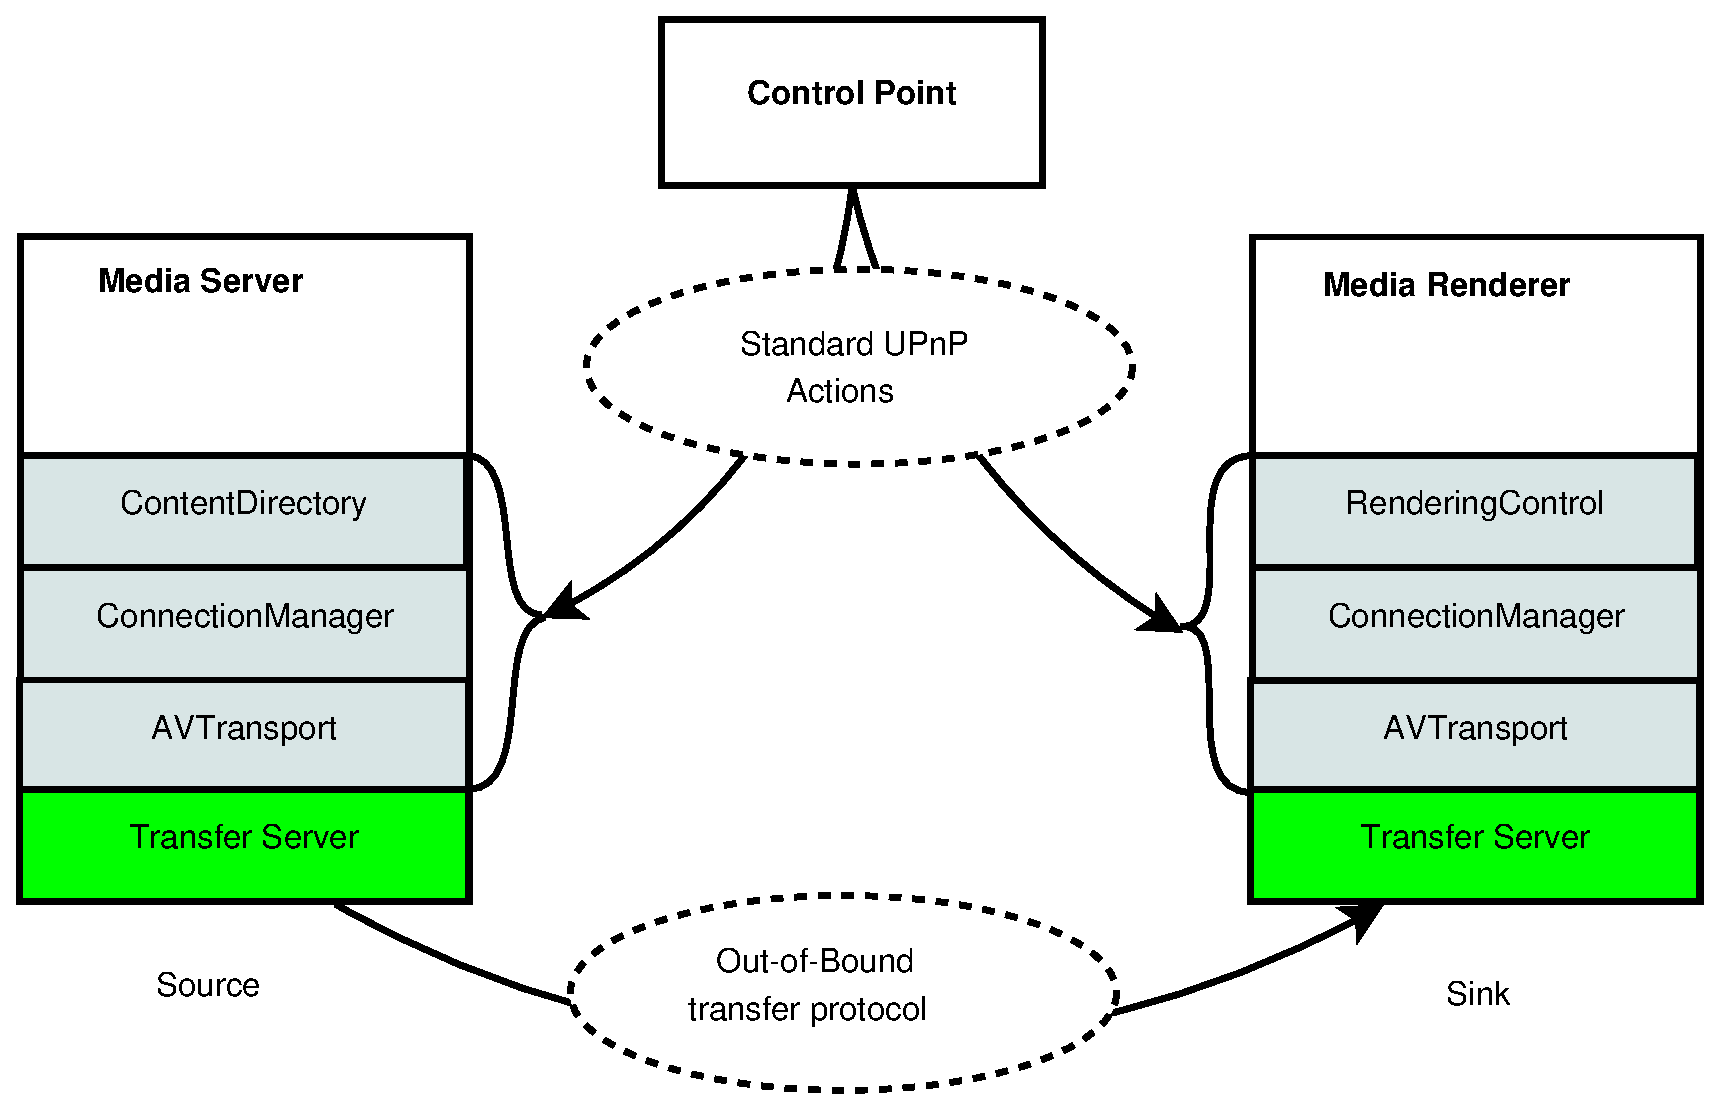
\includegraphics[height=9cm]{charts/upnp_playback} 
\caption{UPnP A/V playback architecture \label{upnp_playback}} 
\end{figure}

The AV control point interacts with two or more UPnP
devices, one of which acts as either a source or a sink. While coordinated by
the AV control point, the devices themselves interact with each other using a
non-UPnP communication protocol. The control point configures the devices as
needed, triggers the flow of content, then gets out of the way.

\textbf{Media Server}

The media server is used to locate available content in the home network. Its 
primary purpose is to allow control points to enumerate (browse or search) 
content items that are available for the user to render. The media server 
contains a ContentDirectory Service (CDS), a ConnectionManager Service (CM) 
, and an optional AVTransport Service (AVT) which depends on the supported 
transfer protocols. Some media servers are capable of transferring multiple 
content items at the same time. 

The ContentDirectory service is used by the control point to enumerate the content 
on the server. The primary action is ContentDirectroy::Browse(). After 
invoking this action, the control point can obtain detailed information of each 
item that the server can provide. This detailed information includes the name, 
the artist, date created, the size and also the transfer protocols and data formats that are
supported for the particular item. By parsing this detailed information, 
the control point is able to distinguish whether the item can be rendered by the 
given media renderer. 

The ConnectionManager service is used to manage the connections between a 
control point and a device. The primary action is 
ConnectionManager:: PrepareForConnection(), which is invoked by the control 
point to prepare the server for an upcoming transfer. This 
action will return the instanceID of an AVTransport service that will be used 
later to control, say to stop, pause, seek, the flow of content. The instanceID is used to distinguish multiple instances of the AVTransport service. Since each instance is associated with a particular connection to the renderer, the instanceID enables multiple renderer support at the same time. When the 
control point needs to disconnect the connection, it will invoke the media 
server's ConnectionManager::ConnectionComplete() action to release the 
connection. When the ConnectionManager::PrepareForConnection() action is not 
implemented, the control point is only able to support a single renderer at a 
time. In this case 0 will be used as InstanceID. 

The AVTransport service is used by the control point to control the playback of the 
content. Operations like Stop, Pause, Seek are supported by this service. However, this 
service is not mandatory and the media server can choose to implement this feature 
according to the supported transfer protocols and data formats. If this service 
is supported, the InstanceID included in each AVTransport action is used to 
distinguish multiple instances of the service. New instances of the AVTransport 
service can be created by ConnectionManager's 
ConnectionManager::PrepareForConnection() action, and new InstanceID is 
allocated to each new service instance. 

\textbf{Media Renderer} 

The media renderer is used to render the content obtained from home 
networking. Its main feature is that it can be discovered by a control point and perform content rendering according to the instructions from the control point. These instructions could control rendering settings such as brightness, contrast, volume, mute, etc. The control of the flow of the content like stop, pause, seek can also be supported depending on the transfer protocol used. The media 
renderer provides three services including the RenderingControl service, the ConnectionManager 
service and an optional AVTransport service. Sometimes the rendering control and 
AVTransport services contain multiple independent instances so that the device 
could be able to handle multiple content items at the same time. Those multiple 
instances can be identified by a unique InstanceID.

The RenderingControl service is used by the control point to control how the renderer 
renders the incoming content. Characteristics like brightness, contrast, 
volume, mute etc, can be controlled by this service. The RenderingControl service 
supports multiple, dynamic instances, which allows a renderer to mix one or 
more items together. Such a dynamic instance could be a Picture-in-Picture
window on a TV or a mixed audio stream. Multiple connections can be
distinguished by their unique InstanceID. 

The ConnectionManager service is used to manage connections associated with a 
device, the primary action is the ConnectionManager::GetProtocolInfo() action. 
The control point can invoke this action to enumerate the transfer protocols and 
data formats supported by the media renderer. By comparing this information with 
the protocol information retrieved from the media server, the control point is able to 
predetermine if a media renderer is capable of rendering a specific item from 
the media server. Optionally, media renderer may also implement the
ConnectionManager::PrepareForConnection() action to prepare itself for an 
upcoming transfer. It can also assign a unique ConnectionID that can be used by 
a 3rd party control point to obtain information about the connections that the media 
renderer is using. In addition, depending on the transfer protocol and data 
format used, this action may also return a unique AVTransport InstanceID that the control 
point can use to control the flow of content (stop, pause, seek, etc). 

The AVTransport service is used to control the flow of streamed content. Actions 
like play, stop, pause and seek can be controlled depending on the transfer 
protocol and supported data formats. The AVTransport service can also support 
multiple logical instances and handle multiple simultaneous content items. The 
AVTransport InstanceID which is used to distinguish service instances can be 
allocated by ConnectionManager::PrepareForConnection(). 
\clearpage
\textbf{Control Point} 

The Control Point is used to bridge communication between a media server and a media renderer. 
It also provides the user interface to users. A control point does not implement UPnP 
services, as a result it is not visible as a device on the network. Usually the control point 
invokes a media server or a media renderer's services in order to complete the 
desired operations.

The user control point can be used in different scenarios. In a typical use
scenario, a control point firstly discovers Audio/Video receiver devices and
media servers. It locates the desired media content on a media server and gets
the renderer's supported protocols and formats, then the control point compares
this information with the desired media content and decides whether the desired
media item can be played on the receiver. If the media format is supported by
the receiver, the control point then configures the media server and media
renderer to prepare for a direct connection. The control point then starts a
content transfer process between the media server and the renderer. During the
media playback, the control point is used to adjust the rendering
characteristics, such as volume, brightness and progress. After the playback,
the control point can either select the next content in the playlist or clean up
the media server and media renderer.

As described above, three basic functional entities are defined in the UPnP AV 
architecture \cite{upnp-av}, which are Media Server, Media Renderer and Control
Point respectively. A physical device can consist of a combination of any of
these functional entities. One typical example is that a DLNA Media player is a
combination of a Control Point and a Media renderer.

A simplified UPnP Audio Video 3-box model \cite{DLNA_proxy} can be 
seen in Figure \ref{av_use_scenario}.
\begin{figure}[htb] 
\centering 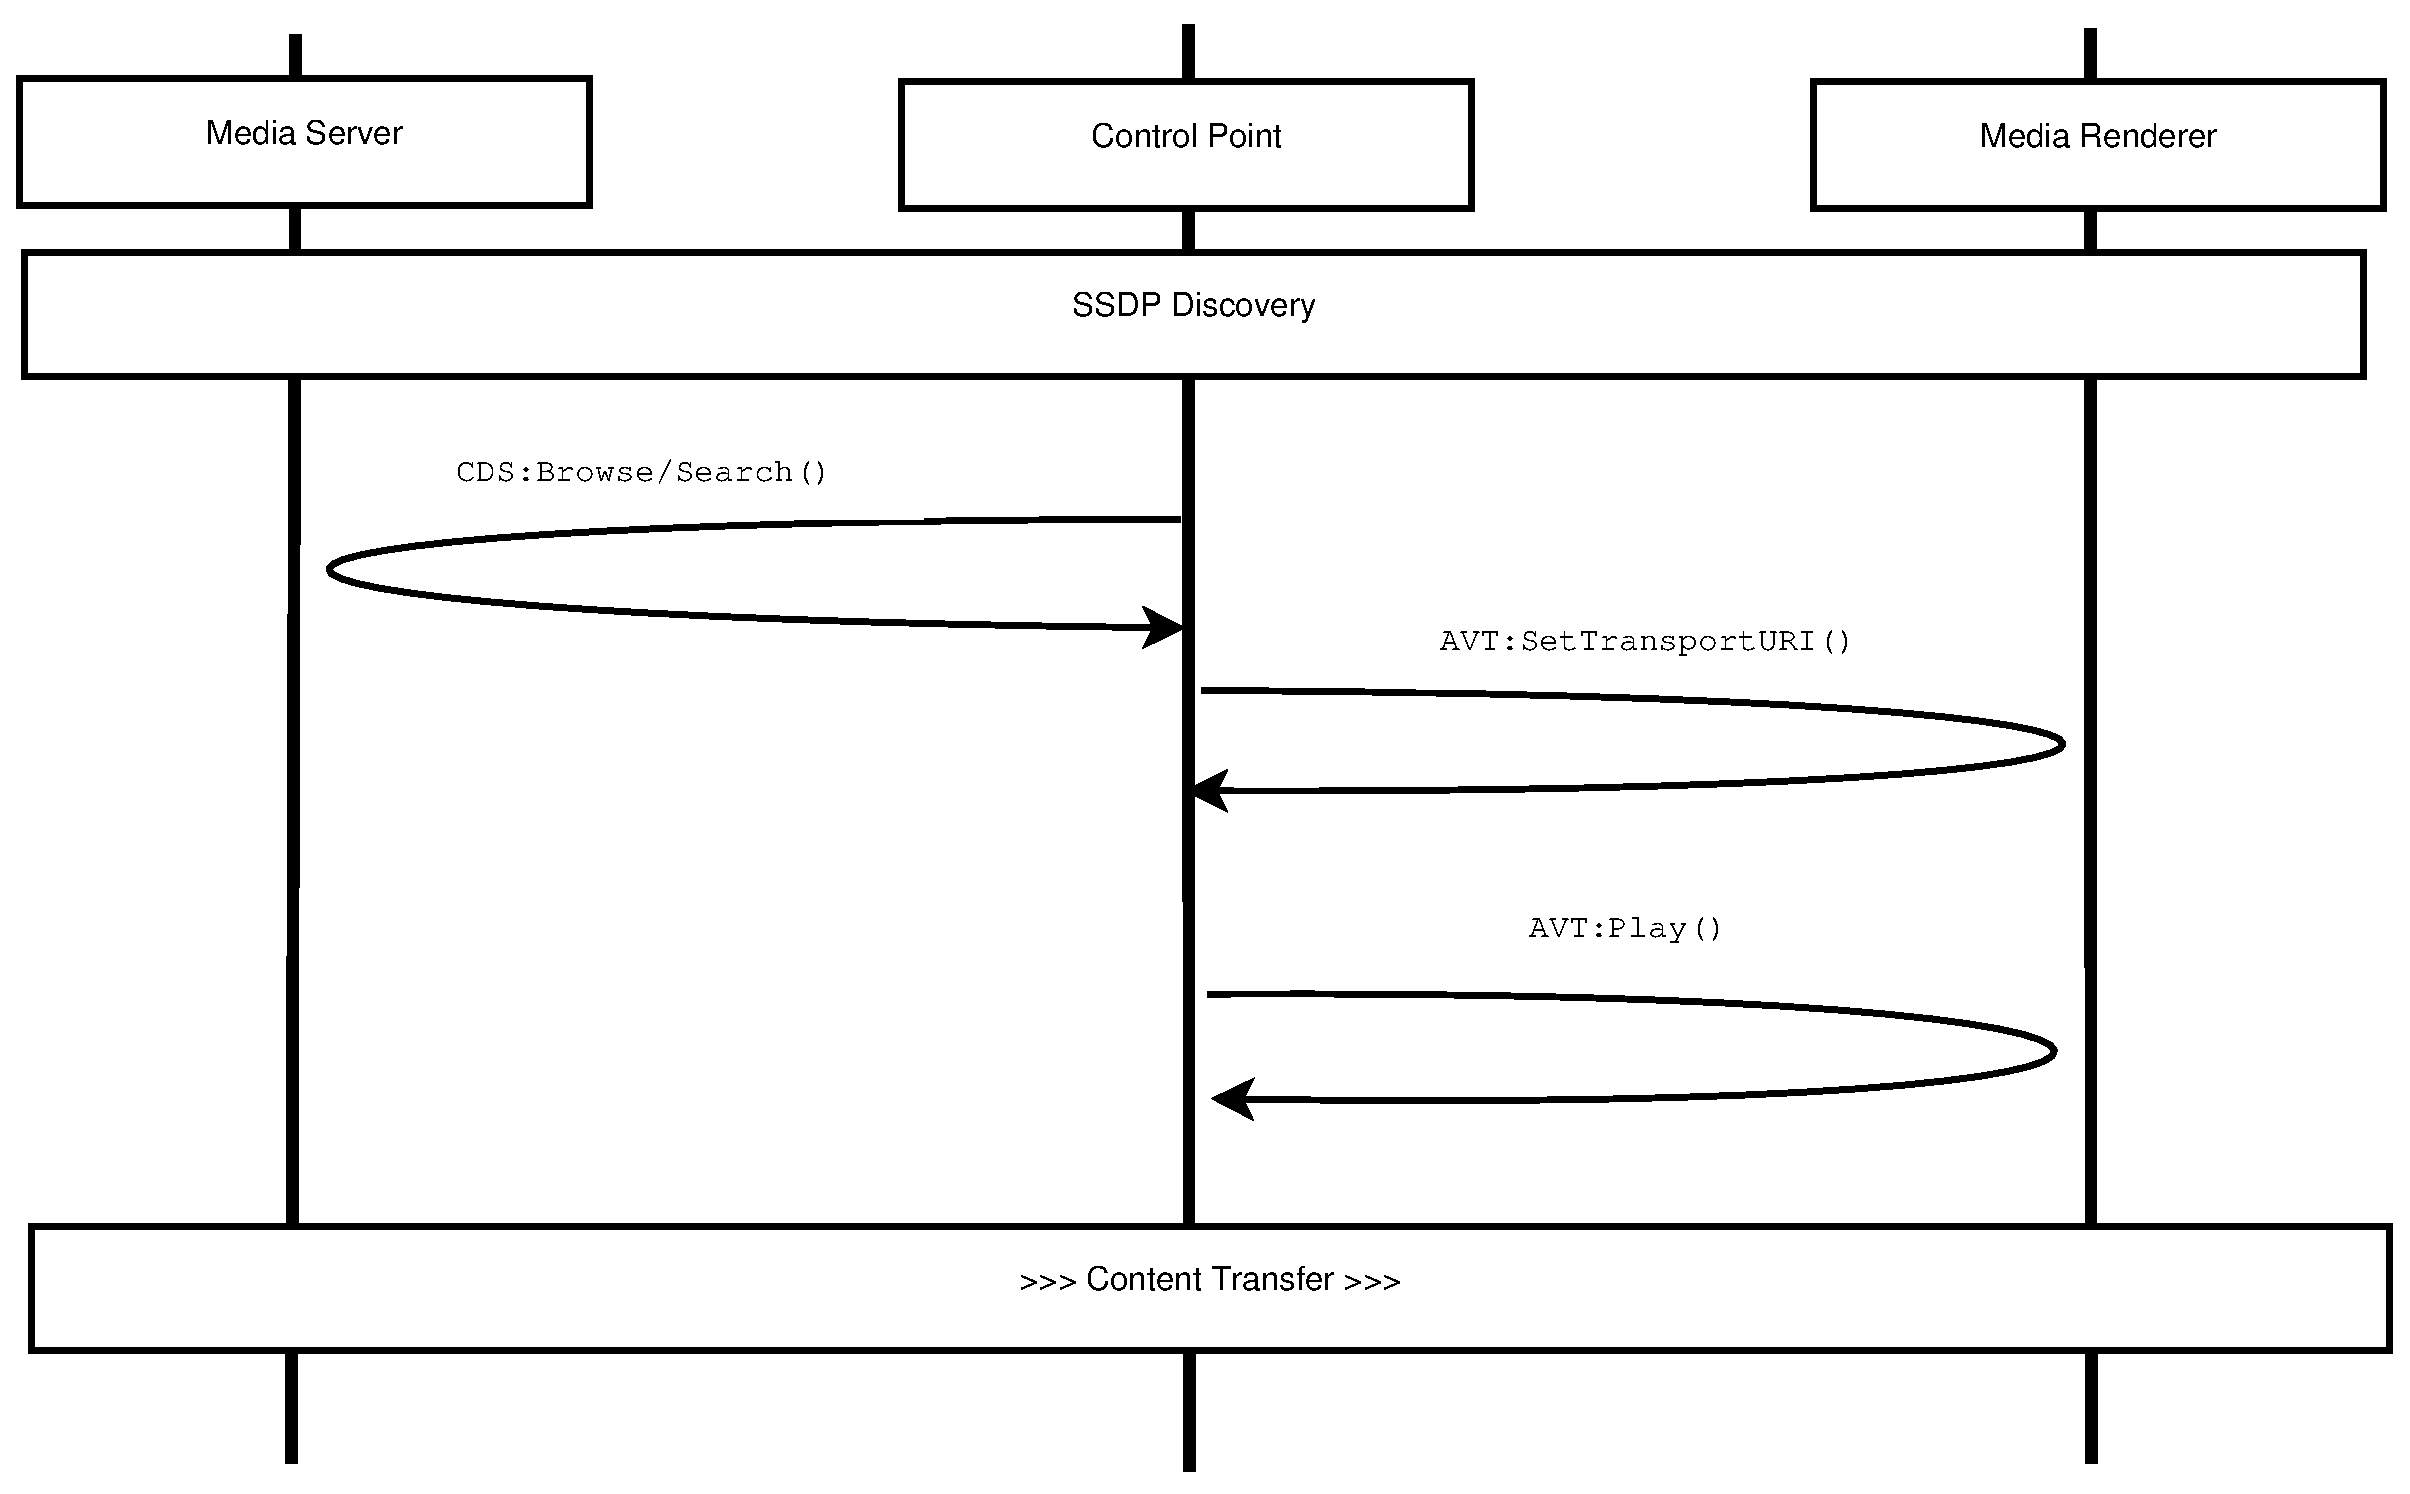
\includegraphics[height=9cm]{charts/chart1} 
\caption{Typical UPnP AV use scenario \label{av_use_scenario}} 
\end{figure} 
The first thing in the UPnP network communication is the Simple Service
Discovery Protocol (SSDP)-based device discovery. A SSDP multicast message is
sent when a new device is added to the network. A control point would listen to these 
multicast messages. On receiving the SSDP message, the control point would send a request for the device's description and services using the location found in the SSDP discovery message. Then the control point can issue the services action command using the Simple Object Access protocol (SOAP).

In media sharing scenarios, the control point would browse the information about 
the Content Directory Service (CDS) provided by the Media Server. A 
browse/Search action can be invoked to navigate through the content stored in 
the Media Server device. After the control point has selected the media content from 
a Media Server, a Media Renderer AVTransport::SetAVTransportURI would be sent by 
the control point to the Media Renderer. Finally, the Play command is invoked by 
the control point to instruct the Media Renderer. Afterward, the transfer begins. The media 
stream travels directly between the Media Server and the Media Renderer, through HTTP, 
RTP \cite{rtp_rfc} or other streaming protocols.

The media playback control actions can also be invoked by the control point. Methods 
supported include volume control, seek, pause etc. 

\subsection[DLNA]{Digital Living Network Alliance\label{2_2_2}} 
DLNA is a relatively old industry standard compared with other home networking 
solutions. It is mainly based on the UPnP Audio/Video architecture, which is 
discussed in section \ref{2_2_1_2} and shown in Figure \ref{upnp_playback}. As a
result, it is widely used by many manufactures. Newer home networking solutions
are also influenced by DLNA and they follow similar technologies used in DLNA.
In this paper the DLNA and UPnP standard architectures are studied to help us
gain a grasp of how a home networking solution could look like.

An overview of the DLNA architecture \cite{dlna_guideline} can be divided into
five parts: Architectures and Protocols, Media Format Profiles, Link Protection,
Digital rights management (DRM), Interoperability Solutions (DIS) and Device
Profiles.

\textbf{Architectures and Protocols}

%% table 3, Key Technology Ingredients 
\begin{table}[htb] 
\caption{Key Technology Ingredients\label{dlna_key_tech} \cite{dlna_guideline}} 
\begin{center} 
\fbox{ 
\begin{tabular}{c|c}  
\textbf { Functional Components } & { Technology Ingredients } \\ \hline 
\textbf Connectivity & Ethernet, 802.11 (including Wi-Fi Direct) \\ 
\textbf  & MoCA, HPNA and Bluetooth \\ \hline 
\textbf Networking & IPv4 Suite \\ \hline 
\textbf Device Discovery and Control & UPnP* Device Architecture v1.0 
\ref{upnpdevice} \\ \hline 
\textbf Media Management and Control & UPnP AV and UPnP Printer:1 
\ref{upnpav}\\ \hline 
\textbf Media Formats & Required and Optional Format Profiles \\ \hline 
\textbf Media Transport & HTTP(Mandatory), HTTP Adaptive \\
\textbf  & Delivery(DASH) and RTP \\ \hline 
\textbf Remote User Interface & CEA-2014-A 
\end{tabular} 
} 
\end{center} 
\end{table} 

The DLNA architecture is built upon the UPnP protocol, which is discussed in
\ref{upnp}. As shown in Table \ref{dlna_key_tech}, in the network layer DLNA
uses the IPv4 suite. On top of the network layer, the UPnP device architecture and UPnP AV architecture are used in DLNA to control
and manage media devices. The DLNA guideline also addresses the media format
compatibility and media transport interoperability issues in support of
interoperability among devices.

\textbf{Media Format Profiles}

DLNA defines the media formats used by the DLNA home networking 
standard. There are three types of media in DLNA: music, video and photo.\\
For music, the minimal requirement is the LPCM format. Used by PCM raw data,
this format is not compressed and it does not require heavy CPU usage. However,
the bandwidth consumption is considerably bigger than in other formats. MP3 is
the most popular music format. It is a compressed format and requires some CPU
power for encoding and decoding. Compared with LPCM, the bandwidth consumption
of MP3 is less, making it suitable for low bandwidth networking. AAC is another
kind of compressed audio format and it became popular since it is the default
media format of iTunes. It has similar characteristics as MP3.

For photos, the minimal requirement in the DLNA guideline is the JPEG format. In
many occasions JPEG is the only suggested format due to its proven quality and
compress ratio.

For videos, the minimal requirement in DLNA guideline is the MP4 format. The
detailed audio and video codecs are also specified in DLNA media format
guidelines. In a device-to-device scenario, the media server may store a huge
amount of differently formatted media. The communication between two devices
should follow the same encoding mechanism. Normally the media server takes the
responsibility to transcode the media to a certain format defined by the DLNA
media format profile guideline.

\textbf{Link Protection}

DLNA Link Protection is defined as the protection of a content stream between two 
devices on a DLNA network against illegitimate observation or interception.

Content protection is an important mechanism to ensure that commercial content is protected 
from piracy and illegitimate redistribution. Link Protection is a technique that enables the
distribution of protected commercial content on a home network. It provides
protection for copyright holders and content providers without sacrificing
consumer flexibility.
\clearpage
\textbf{Digital rights management (DRM) Interoperability Solutions (DIS) }

DIS is intended to be used to enable the secure transfer and use of protected 
commercial content among different implementations on network media devices. 
The content could be protected by different content protection technologies, 
which are described as DRMs in short.

\textbf{Device Profiles}

A Device Profile is a collection of DLNA capabilities and features within a DLNA device. For a device 
to be compliant with a Device Profile, it has to conform to all of the guidelines listed for that 
Device Profile.

In practice, Device Profiles reference existing optional or recommended DLNA guidelines that enable certain features, and makes those DLNA guidelines mandatory within the context of a Device Profile. 
A Device Profile can also provide some additional guidelines that complement or
modify existing DLNA guidelines for a feature.

A particular type of DLNA Device Profile is the Commercial Video Profile (CVP).
A CVP Device Profile is an extension of the DLNA guidelines that will allow
content from service providers and multichannel video programming distributors
to be distributed on the DLNA network. DLNA Commercial Video Profiles (CVPs)
are defined as Device Profiles that consistently enable commercial content that
enters the home network through a gateway device via an interface to a
commercial content service provider. Since different regions of the world have
different requirements for commercial content, multiple CVPs have been defined.

\subsection{AirPlay\label{2_2_3}} 
AirPlay is Apple Inc's home networking solution. It is a family of protocols 
used to display different types of media content on Apple TV from other iOS devices. 
AirPlay supports multiple functions, including displaying photos and sideshows
from iOS devices, streaming audio from iOS devices or iTunes, as well as
displaying videos from an iOS device and showing the whole screen on Apple TV,
which is known as AirPlay Mirroring.

AirPlay's specification is not open to public. However, unofficial
specifications have been made by some hackers through reverse engineering the
protocol stack. These unofficial specifications could be found on the
Internet\footnote{\url{http://nto.github.io/AirPlay.html}}.
Figure \ref{airplay_use_scenario} shows the playback architecture
of AirPlay. The AirPlay specification includes 6 parts, including service discovery, video
streaming, photo streaming, music streaming, screen mirroring and
authentication.
\clearpage
\begin{figure}[htb] 
\centering 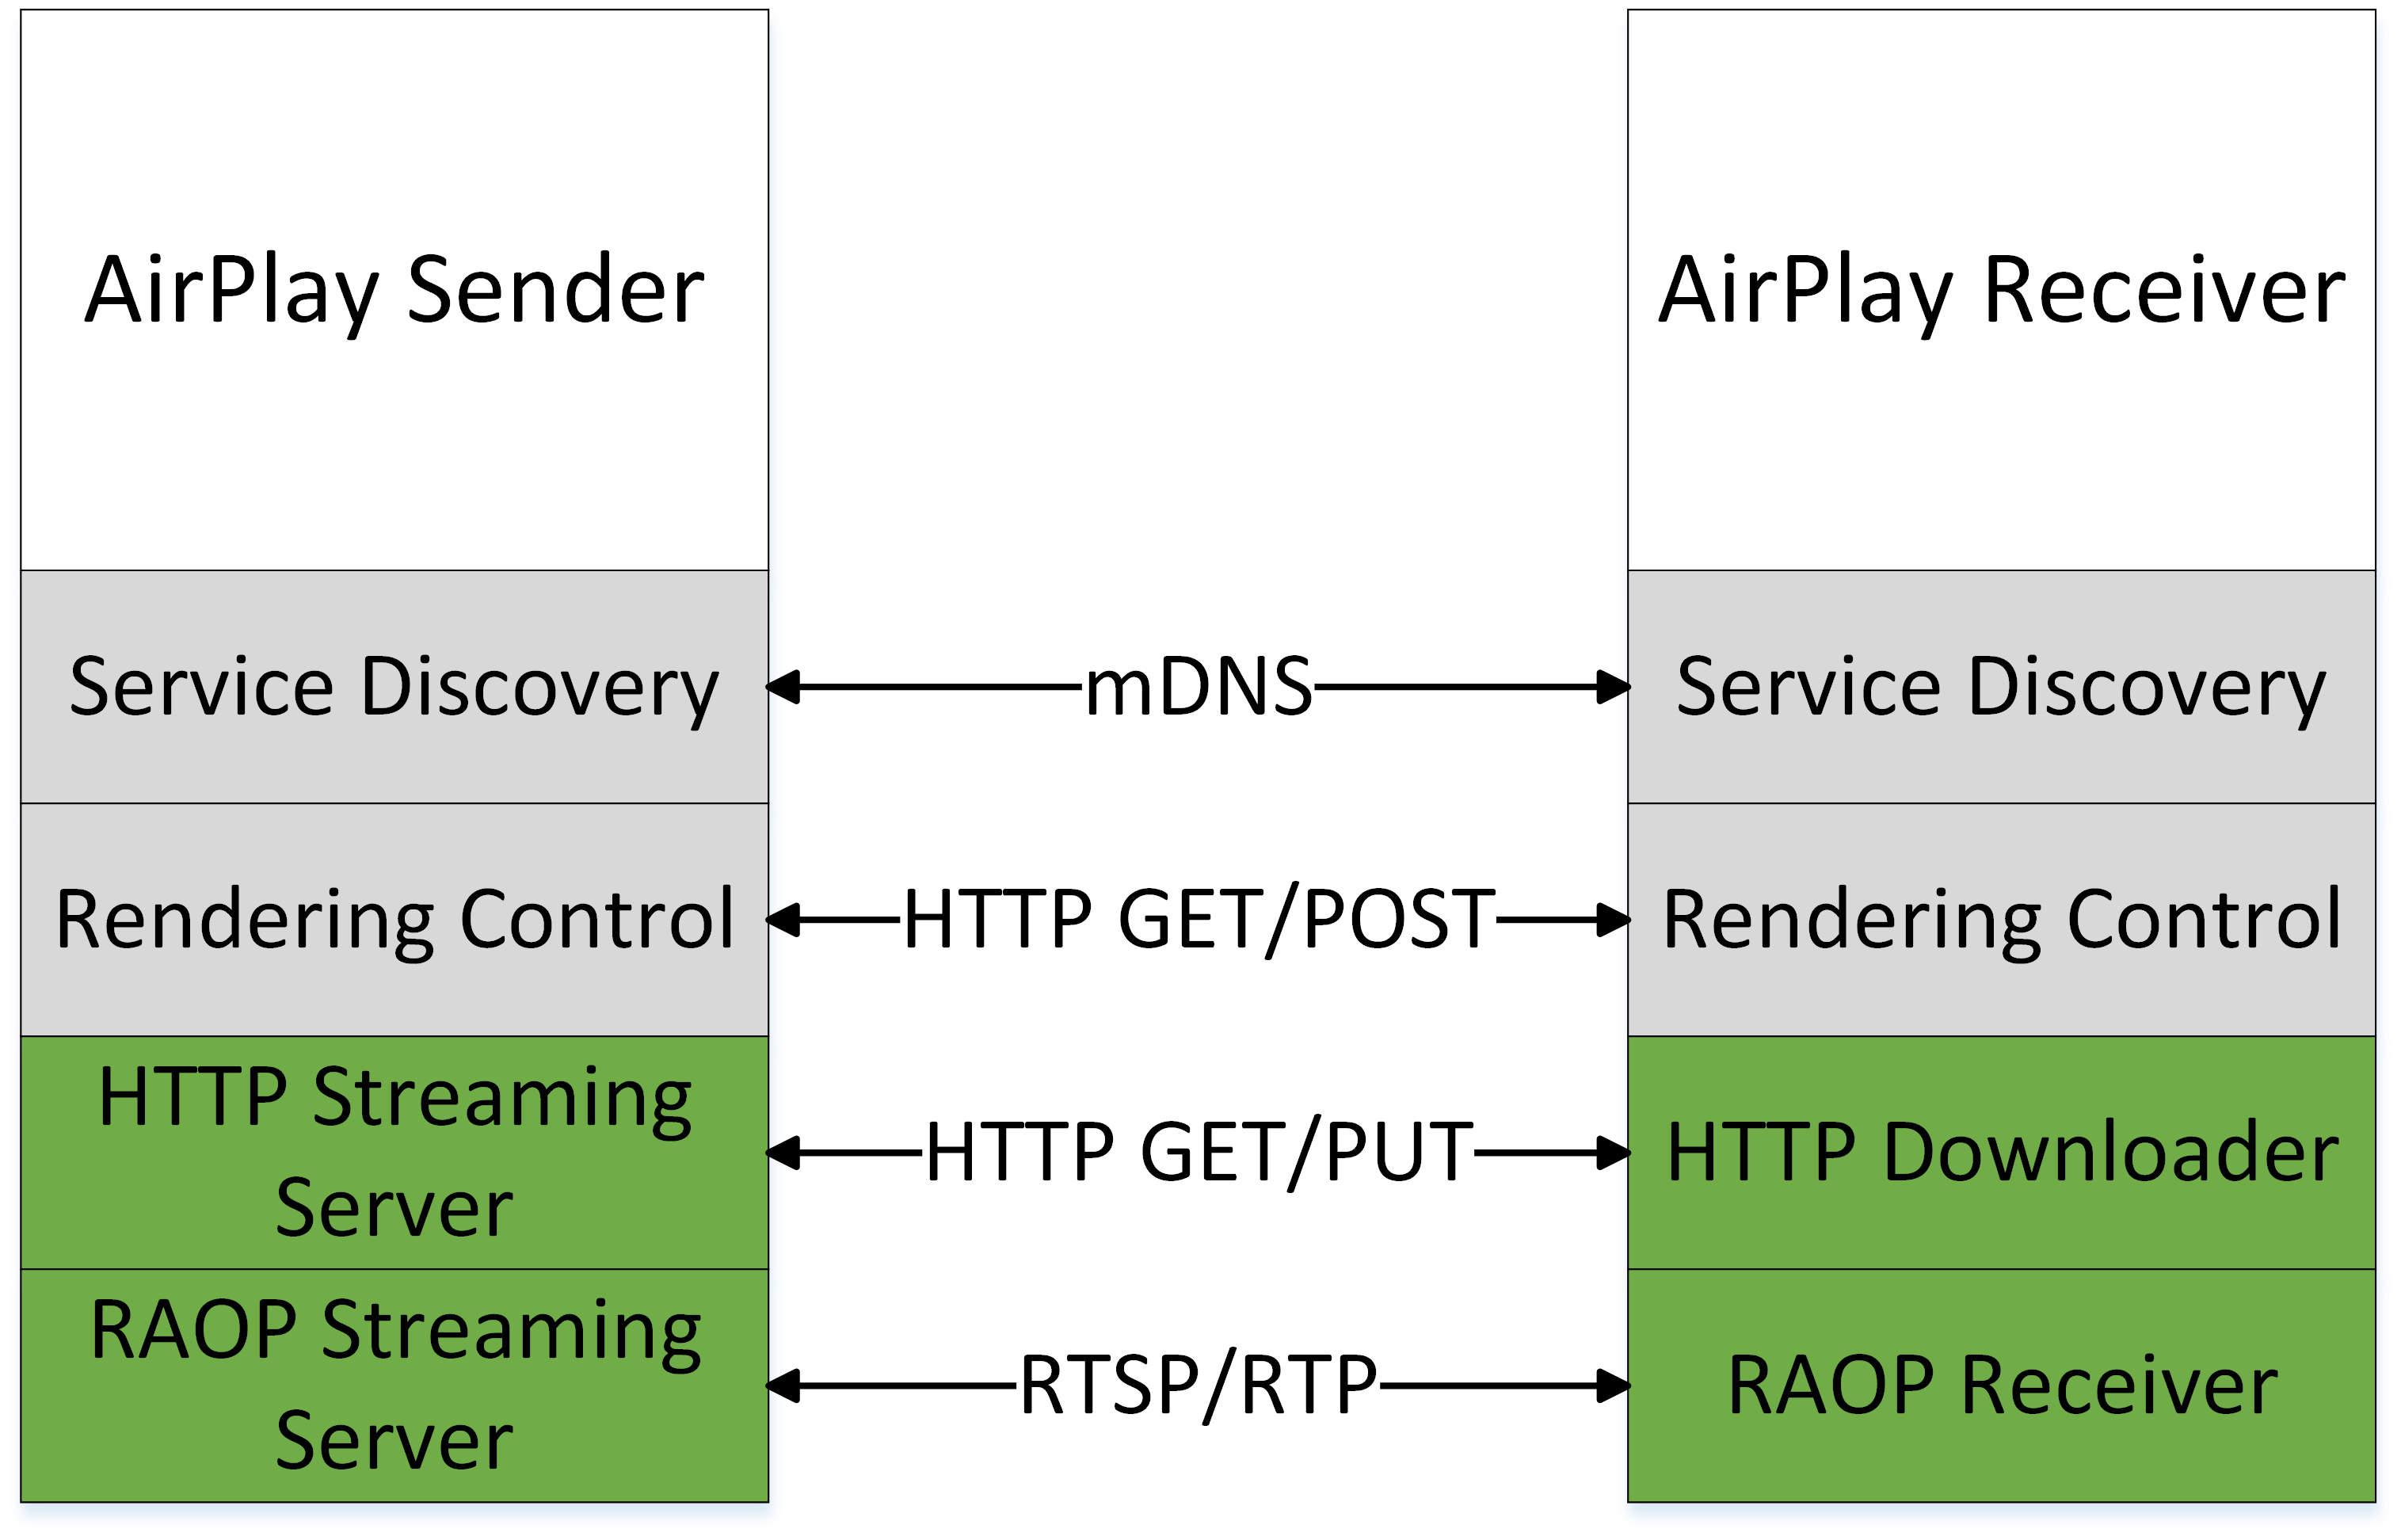
\includegraphics[width=0.7\columnwidth]{charts/airplay} 
\caption{AirPlay playback architecture\label{airplay_use_scenario}} 
\end{figure}  
\textbf{Service discovery}

The service discovery of AirPlay stems from the IETF Zeroconf Working Group, 
that is dedicated to improving the ease-of-use (Zero Configuration) of networks.
The Zeroconf working group has made it possible to make two devices in the 
network to communicate effectively using IP, without requiring a specialist to manually 
configure the network.

AirPlay's service discovery is based on Multicast DNS \cite{multicastdns}, which fulfills the
Zeroconf requirement. Multicast DNS is a way of using familiar DNS programming interfaces, packet formats and operating semantics, in a small 
network where no conventional DNS server has been installed. The requirements 
for Zeroconf name resolution could be met by designing an entirely new 
protocol, since it is better to provide this functionality by making minimal changes 
to the current standard DNS protocol. By using Multicast DNS, most current 
applications need no changes at all to work correctly using mDNS in a Zeroconf network. Besides,
engineers do not have to learn an entirely new protocol. Moreover, current network 
packet capture tools are already capable of  decoding and displaying the DNS packets. Thus they do not 
have to be updated to understand new packet formats.

An AirPlay device such as the Apple TV publishes two services. The first one is 
RAOP (Remote Audio Output Protocol), used for audio streaming. The second 
one is the AirPlay service, used for photos and video content.

The AirPlay server is an HTTP server (RFC 2616). Two connections are made to this 
server, with the second one being used as a reverse HTTP connection. This allows a 
client to receive asynchronous events, such as playback status changes, from a 
server.

\textbf{Video streaming}

The video streaming uses typical HTTP streaming technology, the controller sets 
the streaming URL to Apple TV or other AirPlay receivers. While the URL is set, 
Apple TV starts to download video from the server using the URL and starts 
playing when enough data is buffered. The control messages can be seen in 
table \ref{video_stream}. One thing worth mentioning is that Apple TV does
not support volume control for video
streaming\footnote{\url{http://nto.github.io/AirPlay.html}}.

%% table , Video Streaming 

\begin{table}[htb] 
\caption{AirPlay Video Control HTTP requests \label{video_stream}} 
\begin{center} 
\fbox{ 
\begin{tabular}{ c | l |  p{8.5cm} }%{c|l|l}  
\textbf { Method } & { Request } & { Description }\\ \hline 
\textbf GET & /server-info & Fetch general informations about the AirPlay server \\ \hline 
\textbf POST & /play & Start video playback \\ \hline 
\textbf POST & /scrub & Seek at an arbitrary location in the video \\ \hline 
\textbf POST & /rate & Change the playback rate,0 is paused, 1 is normal \\ 
\hline 
\textbf POST & /stop & Stop playback \\ \hline 
\textbf GET & /scrub & Retrieve the current playback position \\ \hline 
\textbf GET & /playback-info & Retrieve playback informations like position, 
duration\ldots \\ \hline 
\textbf PUT & /setProperty & Set playback property \\ \hline 
\textbf GET & /getProperty & Get playback property 
\end{tabular} 
} 
\end{center} 
\end{table} 

\textbf{Photo streaming}

Image streaming uses the HTTP PUT message to send raw image data to the Apple TV
or other devices. After the whole image is received, the image is then rendered on 
screen. AirPlay also supports slide show, the control messages can be seen in 
table \ref{photo_stream}.

\begin{table}[htb] 
\caption{AirPlay Photo Control HTTP requests \label{photo_stream}} 
\begin{center} 
\fbox{ 
\begin{tabular}{ c | l |  p{7.8cm} }%{c|l|l}  
\textbf { Method } & { Request } & { Description }\\ \hline 
\textbf GET & /slideshow-features & Fetch the list of available transitions for slideshows \\ \hline 
\textbf PUT & /photo & Send a JPEG picture to the server \\ \hline 
\textbf PUT & /slideshows/1 & Start or stop a slideshow session \\ 
\hline 
\textbf POST & /stop & Stop a photo or slideshow session 
\end{tabular} 
} 
\end{center} 
\end{table} 
\clearpage
\textbf{Music streaming}

AirPlay music streaming is a bit different from video and image streaming. The 
technology used is the RTSP streaming protocol, which is more of a "push like"
protocol. Different than HTTP streaming where the server responds to a request,
the RTSP streaming server actively pushes UDP packets to the receiver. However,
Apple does not use the standard RTSP but instead uses its own implementation of
RTSP, which is called RAOP (Remote Audio Output
Protocol)\footnote{\url{http://nto.github.io/AirPlay.html}}.
The control messages of RAOP can be seen in table \ref{music_stream}.

\begin{table}[htb] 
\caption{AirPlay Audio Control RTSP requests \label{music_stream}} 
\begin{center} 
\fbox{ 
\begin{tabular}{c|l}  
\textbf { RTSP request } & { Description }\\ \hline 
\textbf OPTIONS & Ask the RTSP server for its supported methods \\ \hline 
\textbf ANNOUNCE & Tell the RTSP server about stream properties using SDP \\ 
\hline 
\textbf SETUP & Initialize a record session \\ \hline 
\textbf RECORD & Start the audio streaming \\ \hline 
\textbf FLUSH & Stop the streaming \\ \hline 
\textbf TEARDOWN & End the RTSP session 
\end{tabular} 
} 
\end{center} 
\end{table} 

\textbf{Screen mirroring}

AirPlay screen mirroring is achieved by transmitting an H.264 encoded video stream 
over a TCP connection. The stream is packeted with a
128-byte header. The audio uses the AAC-ELD format and is sent using the AirTunes protocol. 
The Network time protocol (NTP) \cite{ntp_rfc} is used for synchronization and
the synchronization takes place on UDP port 7010 (client) and 7011 (server). The 
AirPlay server runs a NTP client. Requests are sent to an AirPlay client every 3 
seconds. The reference time stamp marks the beginning of the 
mirroring session. The control messages can be seen in table 
\ref{mirroring_stream}.

\begin{table}[htb] 
\caption{AirPlay Mirroring Control HTTP requests \label{mirroring_stream}} 
\begin{center} 
\fbox{ 
\begin{tabular}{c|l|l}  
\textbf { Method } & { Request } & { Description }\\ \hline 
\textbf GET & /stream.xml & Retrieve information about the server capabilities 
\\ \hline 
\textbf POST & /stream & Start the live video transmission 
\end{tabular} 
} 
\end{center} 
\end{table} 

\textbf{Authentication}

An AirPlay server can require a password for displaying any content from the 
network. It is implemented using standard HTTP Digest Authentication
\cite{http_auth_rfc}, over RTSP \cite{rtsp_rfc} for AirTunes, and HTTP
\cite{http_rfc} for everything else.
The digest realms and user names accepted by Apple TV are described in table \ref{hda}. 

%% table , AirPlay Authentication 
\begin{table}[htb] 
\caption{AirPlay HTTP Digest Authentication \label{hda}} 
\begin{center} 
\fbox{ 
\begin{tabular}{c|c|c}  
\textbf { Service } & { Realm } & { Username }\\ \hline 
\textbf AirTunes & roap & iTunes \\ \hline 
\textbf AirPlay & AirPlay & AirPlay 
\end{tabular} 
} 
\end{center} 
\end{table} 

\subsection{DIAL\label{2_2_4}} 
Chromecast and FireTV use the DIAL \cite{dial} (DIscovery And Launch) standard,
co-developed by Netflix and YouTube, to search for available devices on a Wi-Fi network. 
Once a device is discovered, the protocol synchronizes information on how to 
connect to the device. The protocol is proposed by Google and Netflix, and
consequently YouTube and Netflix already have implemented their DIAL
applications. The streaming part uses HTTP streaming, which means a controller can directly set
the streaming URL and the receiver will start downloading automatically.

As shown in Figure \ref{DIAL_use_scenario}, the DIAL protocol has two
components: DIAL Service Discovery and the DIAL Representational State Transfer
(REST) Service \cite{dial}. DIAL Service Discovery enables a DIAL client device
to discover DIAL servers on its local network and gain access to the DIAL REST
Service on those devices. The DIAL REST Service enables a DIAL client to query,
launch, and optionally stop applications on a DIAL server device. 

The DIAL protocol is based on cloud, so each receiver is a DIAL application
implemented by the content providers. While connecting, the sender application
sends the application ID to the receiver device, which will trigger
the download of the receiver application from cloud. Afterwards, the multimedia
content is directly streamed from the cloud.

\begin{figure}[htb] 
\centering 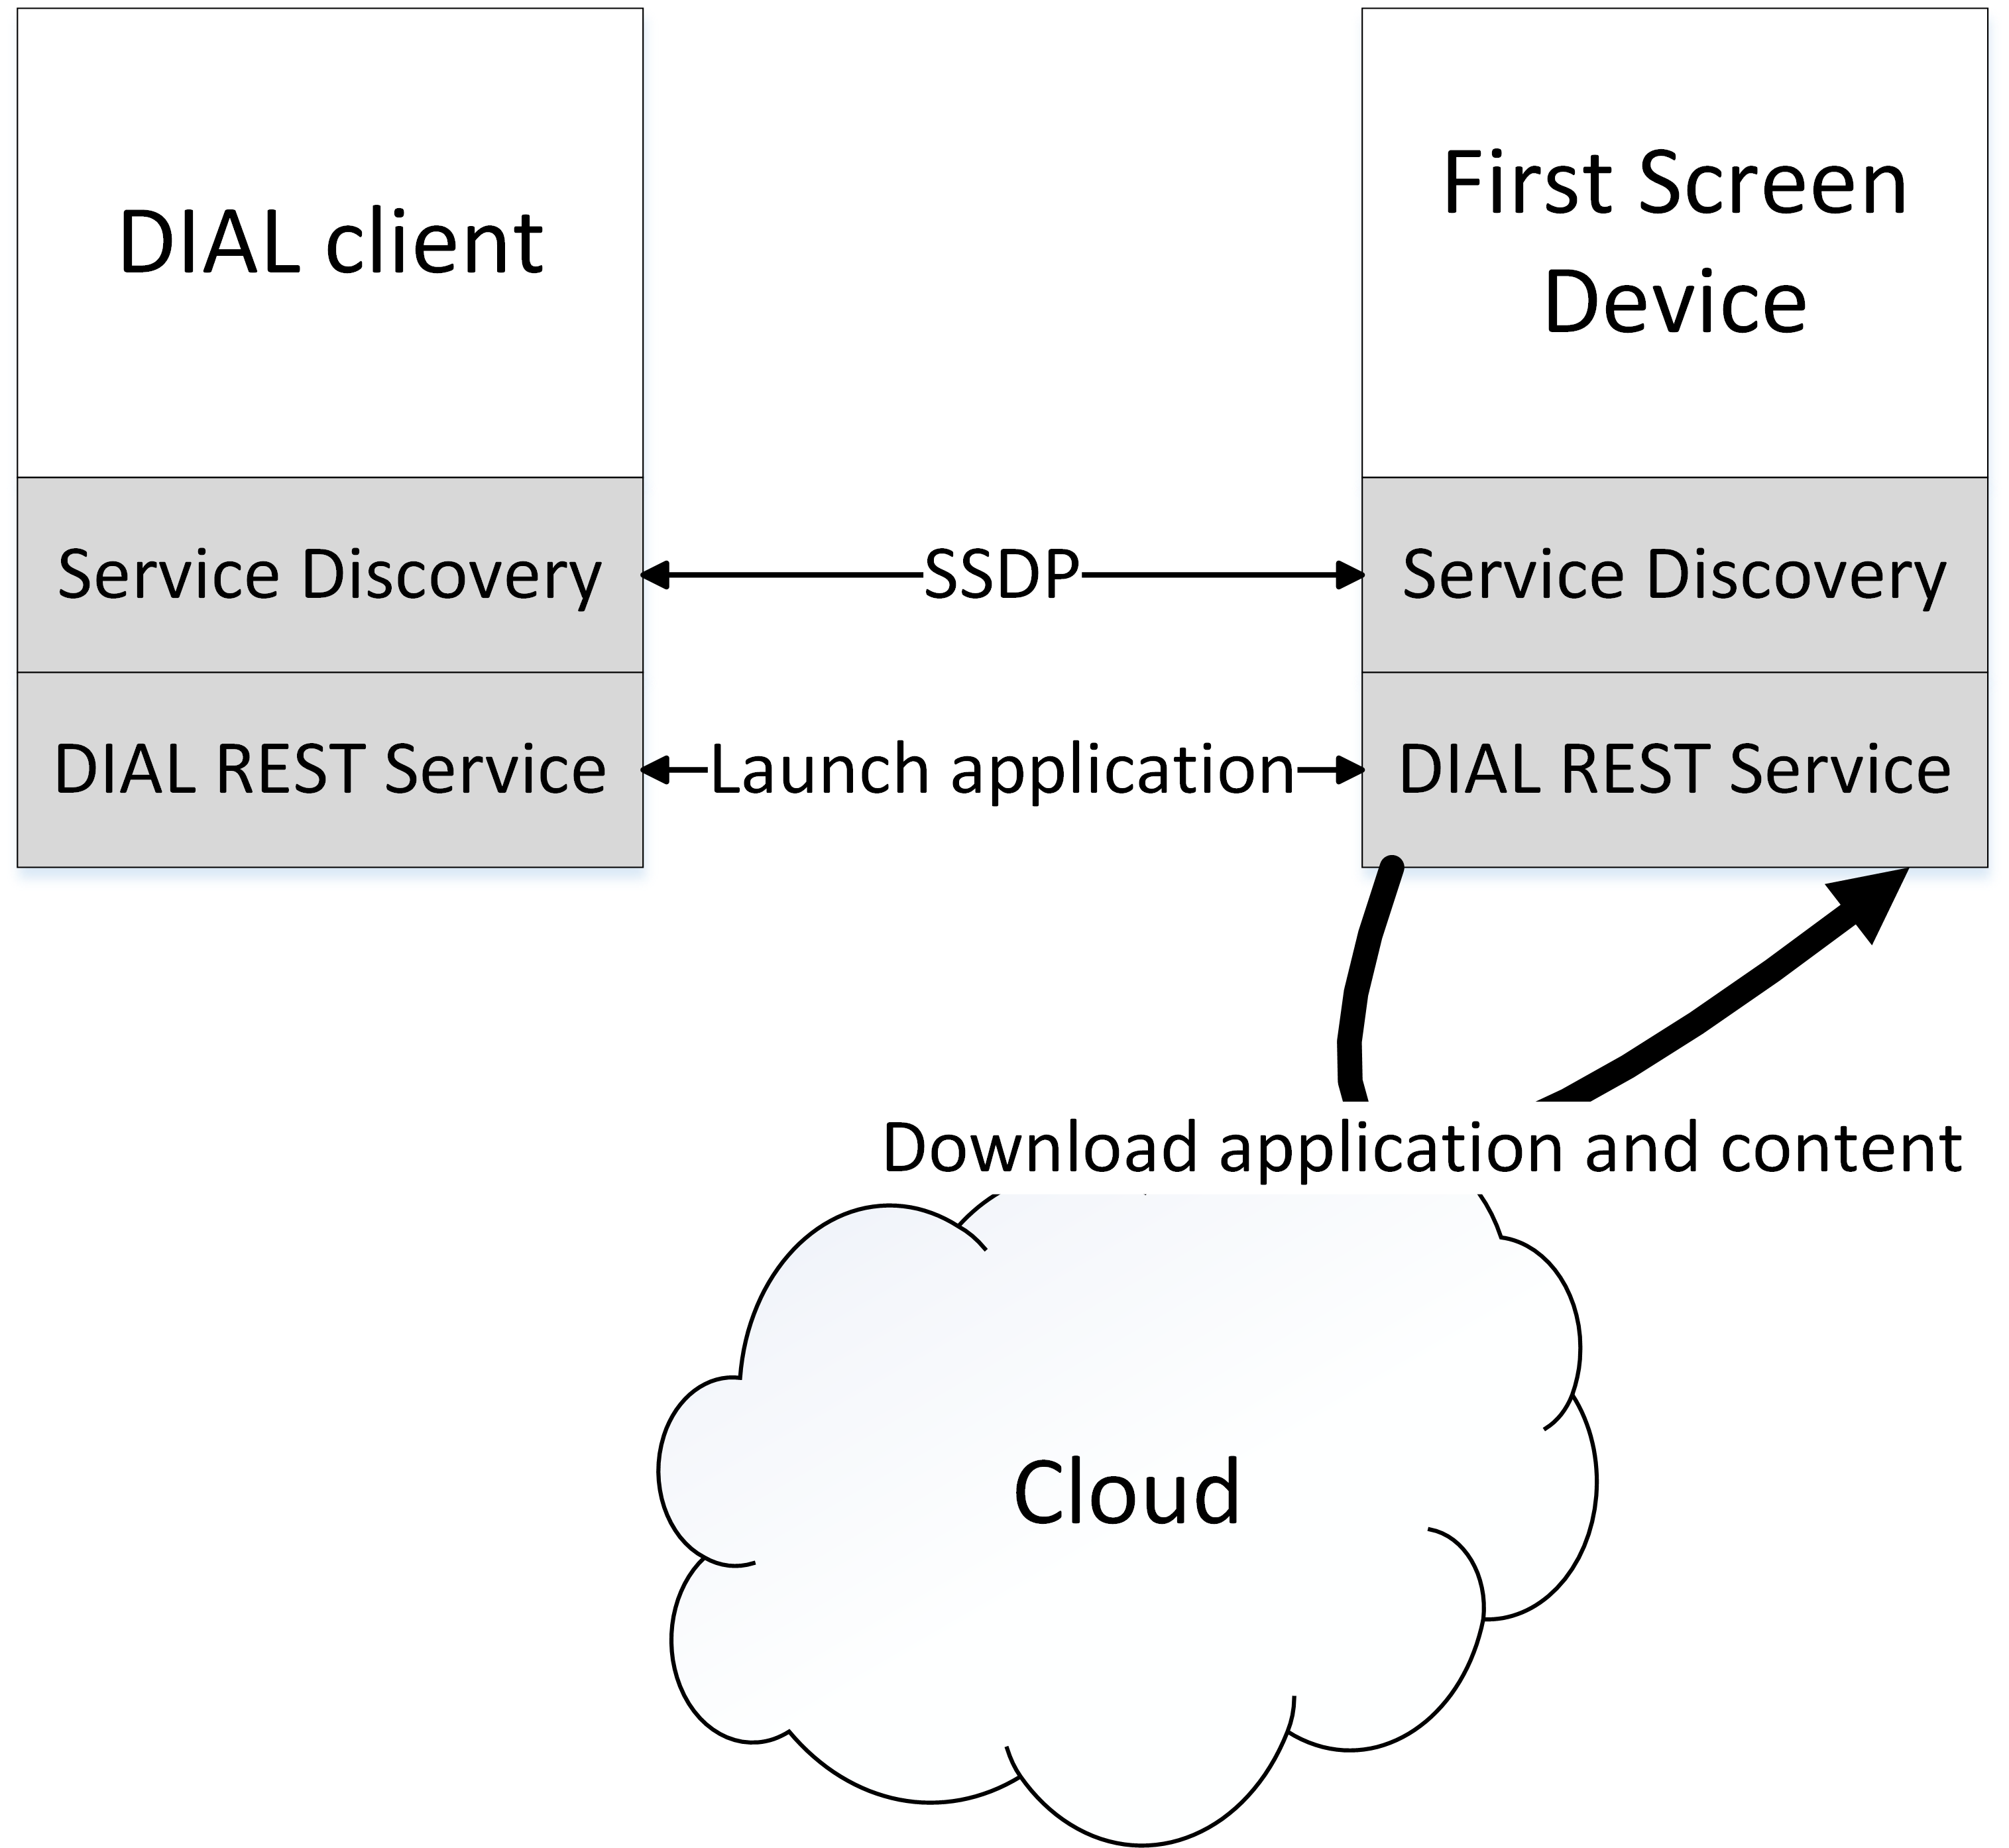
\includegraphics[width=0.7\columnwidth]{charts/DIAL} 
\caption{DIAL playback architecture\label{DIAL_use_scenario}} 
\end{figure}  

\textbf{DIAL Service Discovery}

The DIAL Service Discovery protocol is based on Simple Service Discovery 
Protocol (SSDP) \cite{ssdp_rfc}, which is defined as part of UPnP device
architecture discussed in \ref{upnp}.

\begin{figure}[htb] \centering 
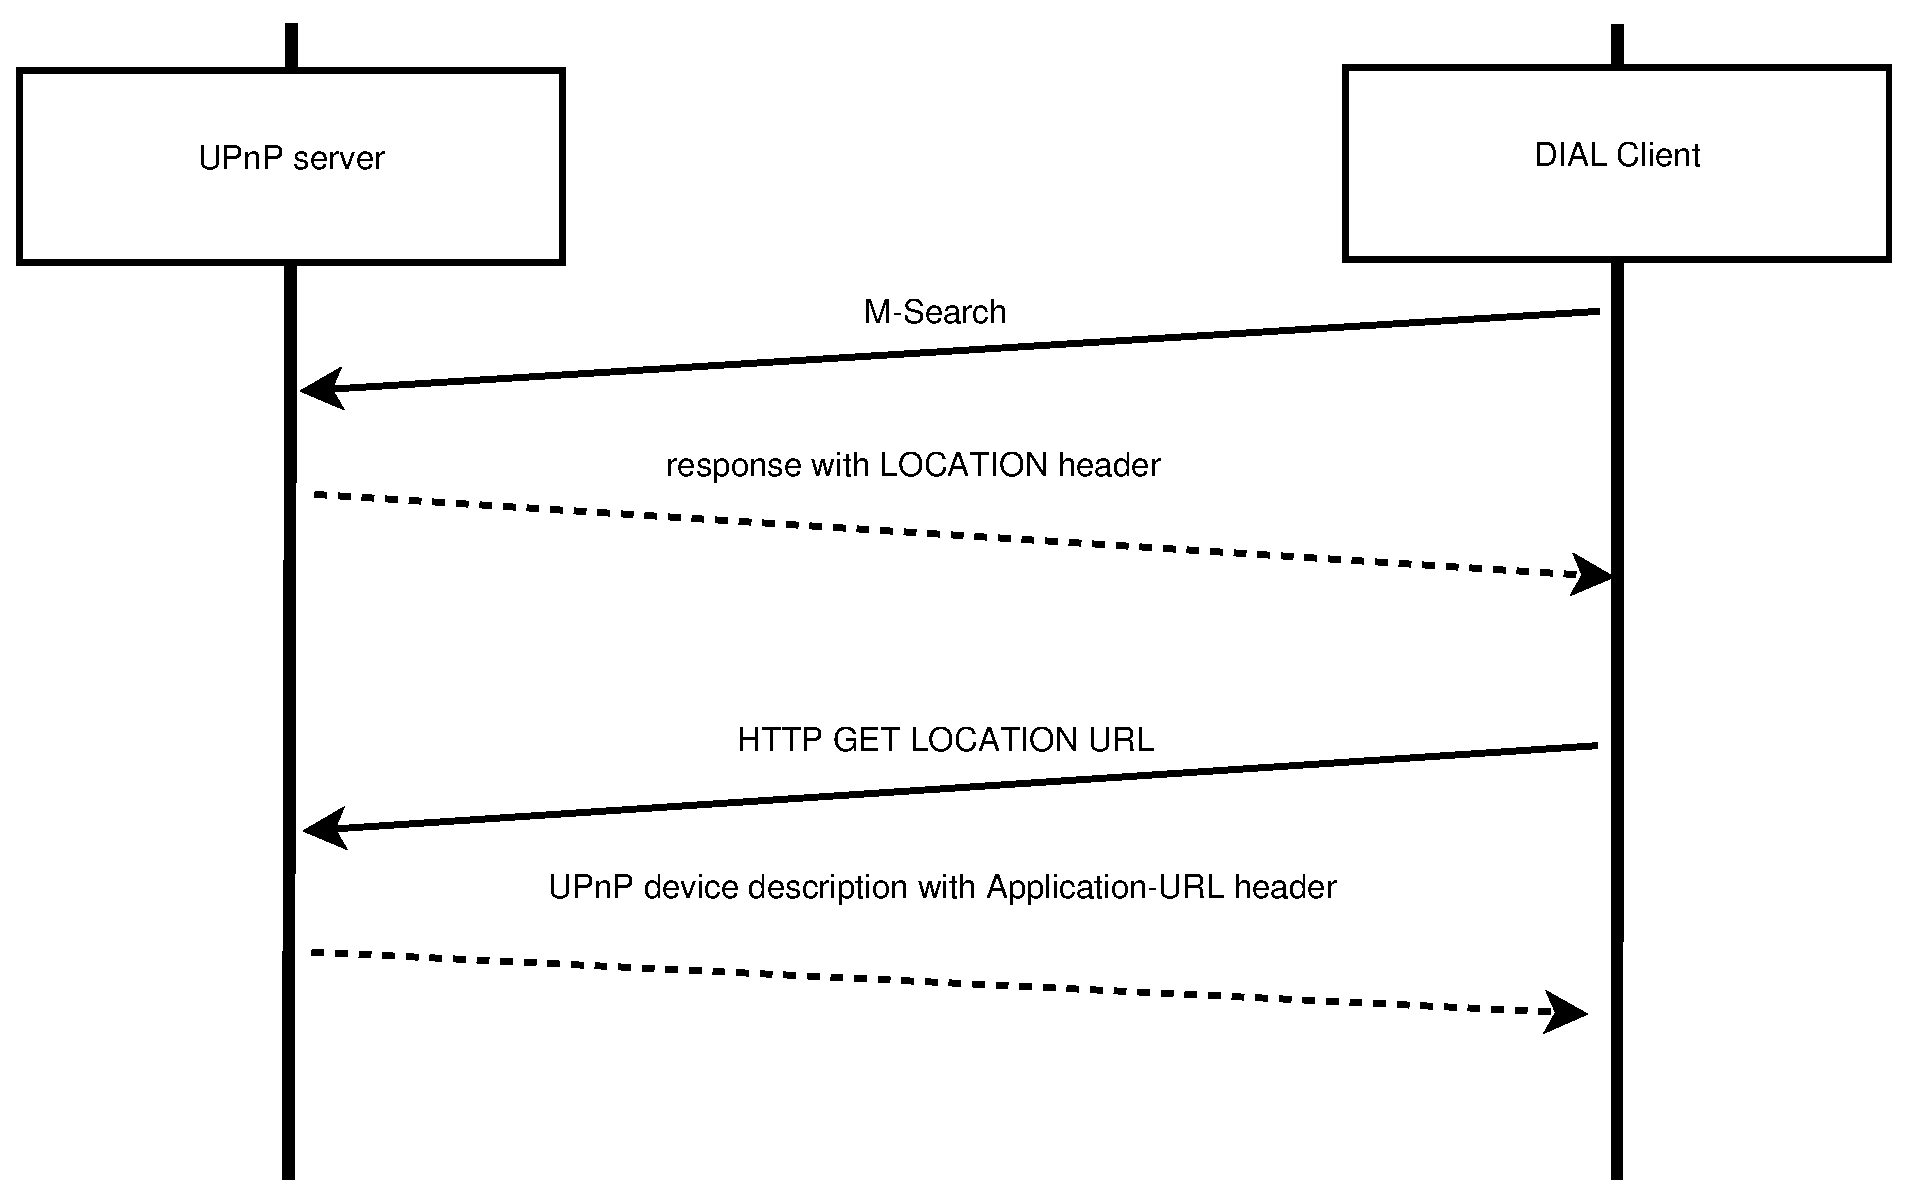
\includegraphics[width=0.95\columnwidth]{charts/dial_discovery} 
\caption{DIAL Discovery \label{dial_discovery}} 
\end{figure} 

The overall flow of DIAL discovery is shown in Figure \ref{dial_discovery}. A
DIAL client will firstly send an M-Search request, which includes  the Search
Target header, over UDP to the IPv4 multicast address 239.255.255.250 and UDP
port 1900. After that the SSDP/UPnP server responds with a response message
including a LOCATION header containing an absolute HTTP URL for the UPnP
description of the root device. When receiving the M-SEARCH response, the DIAL
client then sends an HTTP GET request to the URL found in the LOCATION header
of the M-SEARCH response, to get a prospected HTTP response message containing
a XML format UPnP device description \cite{dial}. 

\textbf{DIAL REST Service}

The DIAL REST service allocates URLs for different resource applications such as 
YouTube and Netflix. Then the application can be controlled by issuing HTTP 
requests against the URL for that application. The Application resource URL is 
constructed by concatenating the DIAL REST service URL, a single slash character 
('/') and the application name. The application name must be registered in DIAL 
Registry to be used.

A DIAL client sends an HTTP GET request to the application resource URL. 
The server receiving the request then extract the application name and check if the 
application is installed or not. If the application is not recognized, the 
server will either return 404 Not Found or trigger the installation of this specific 
application. If the application has been installed, the DIAL server returns 
an HTTP response with 200 OK and a body contains MIME type in XML \cite{dial}.

The client then sends an HTTP POST request to the application resource URL to 
launch the desired application. On receipt of a valid POST request, the DIAL 
server will extract the application name, run the application, and then send 
an HTTP response with the LOCATION header, to inform the absolute HTTP URL, which 
identifies the running instance of the application.

The first-screen application can also send small amount of data to the DIAL 
server, and then the DIAL server can send the information to DIAL clients. 
After the application is launched and the communication is established, the DIAL 
client can communicate directly with the application. The flow chart of  the
DIAL REST service is  shown in Figure \ref{dial_rest}.
\begin{figure}[htb] \centering 
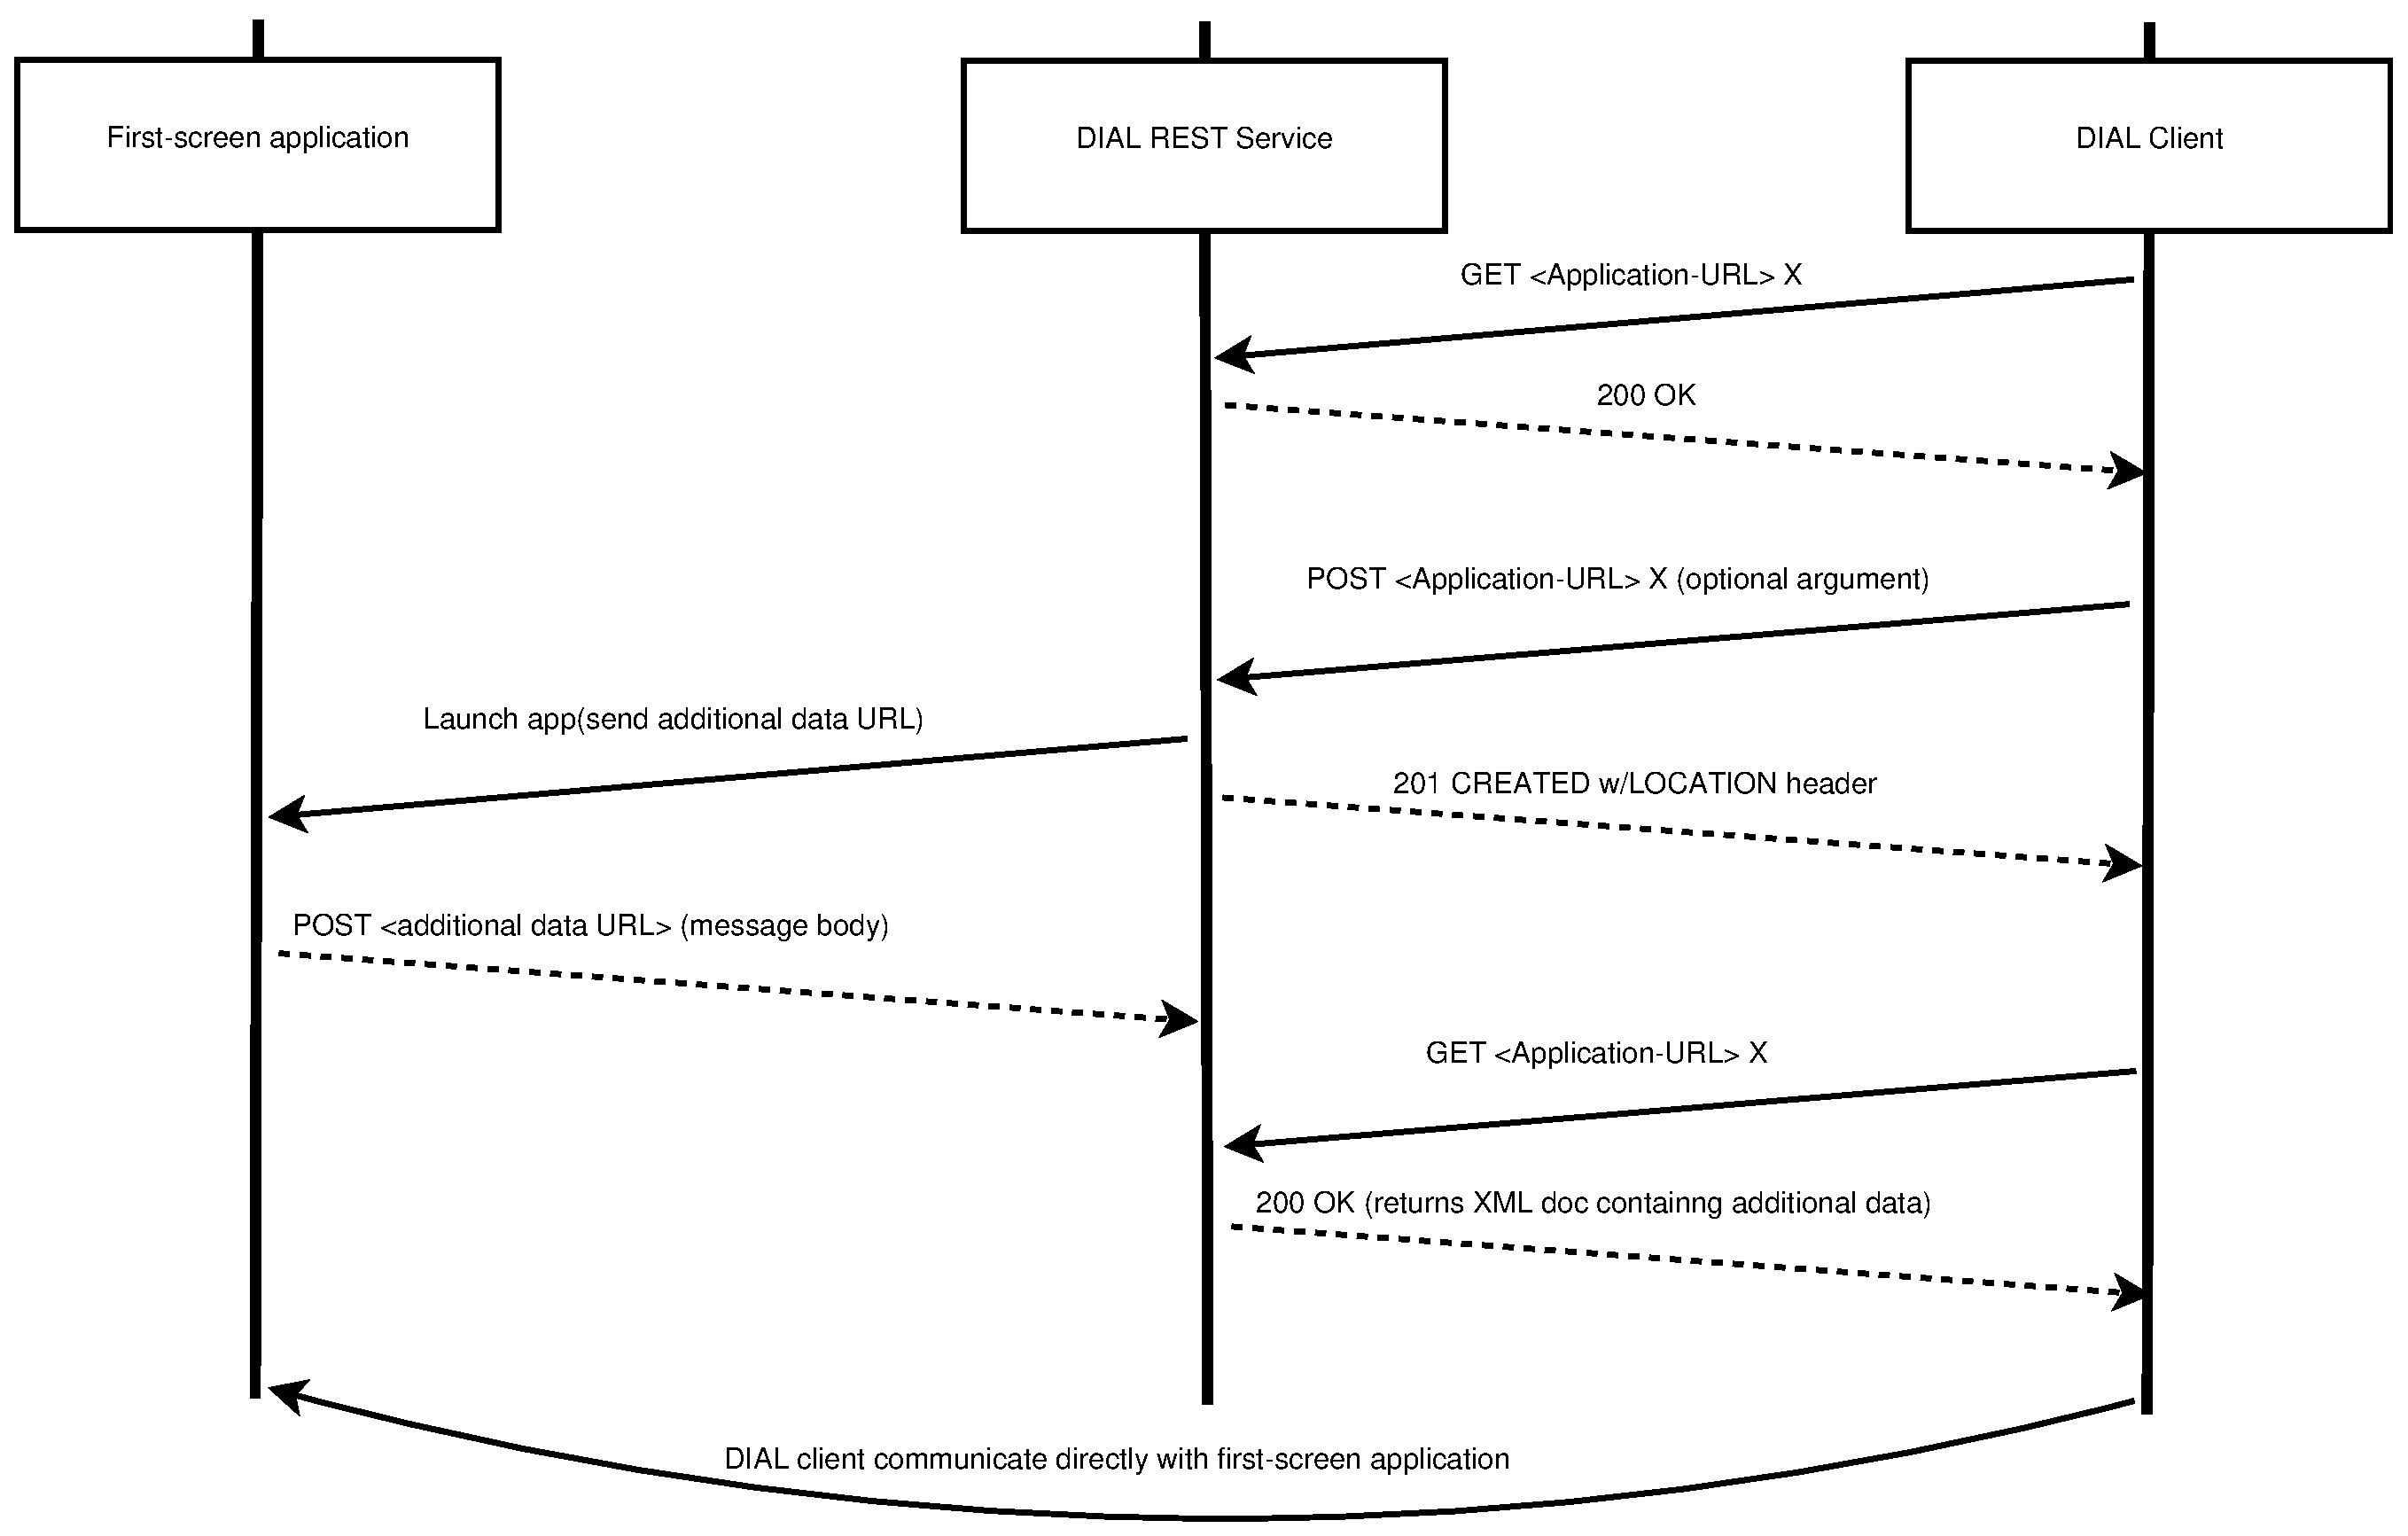
\includegraphics[width=1\columnwidth]{charts/dial_rest} 
\caption{DIAL REST service: application launch \label{dial_rest}} 
\end{figure} 
\clearpage
\subsection{Miracast\label{2_2_5}} %NOT Edited
Miracast \cite{miracast_industry} is very different on technology perspective.
Devices which utilize Miracast technology are not necessarily connected to
the same local network, a Wi-Fi peer to peer connection will be created when
needed. This makes Miracast more adaptive than other technologies, in other
words, Miracast is not limited to the pre-configured network infrastructure.
Figure \ref{miracast_use_scenario} shows the playback architecture of Mircast, the
service discovery is based on Wi-Fi Direct technology. After the connection to
the receiver device is established, the whole screen of the sender device is
recorded and transferred to the receiver device in real time. If the streamed
content is located in the cloud, the content will be firstly downloaded and
displayed on the sender's screen, and then transferred to the receiver device in
real time.

\begin{figure}[htb] 
\centering 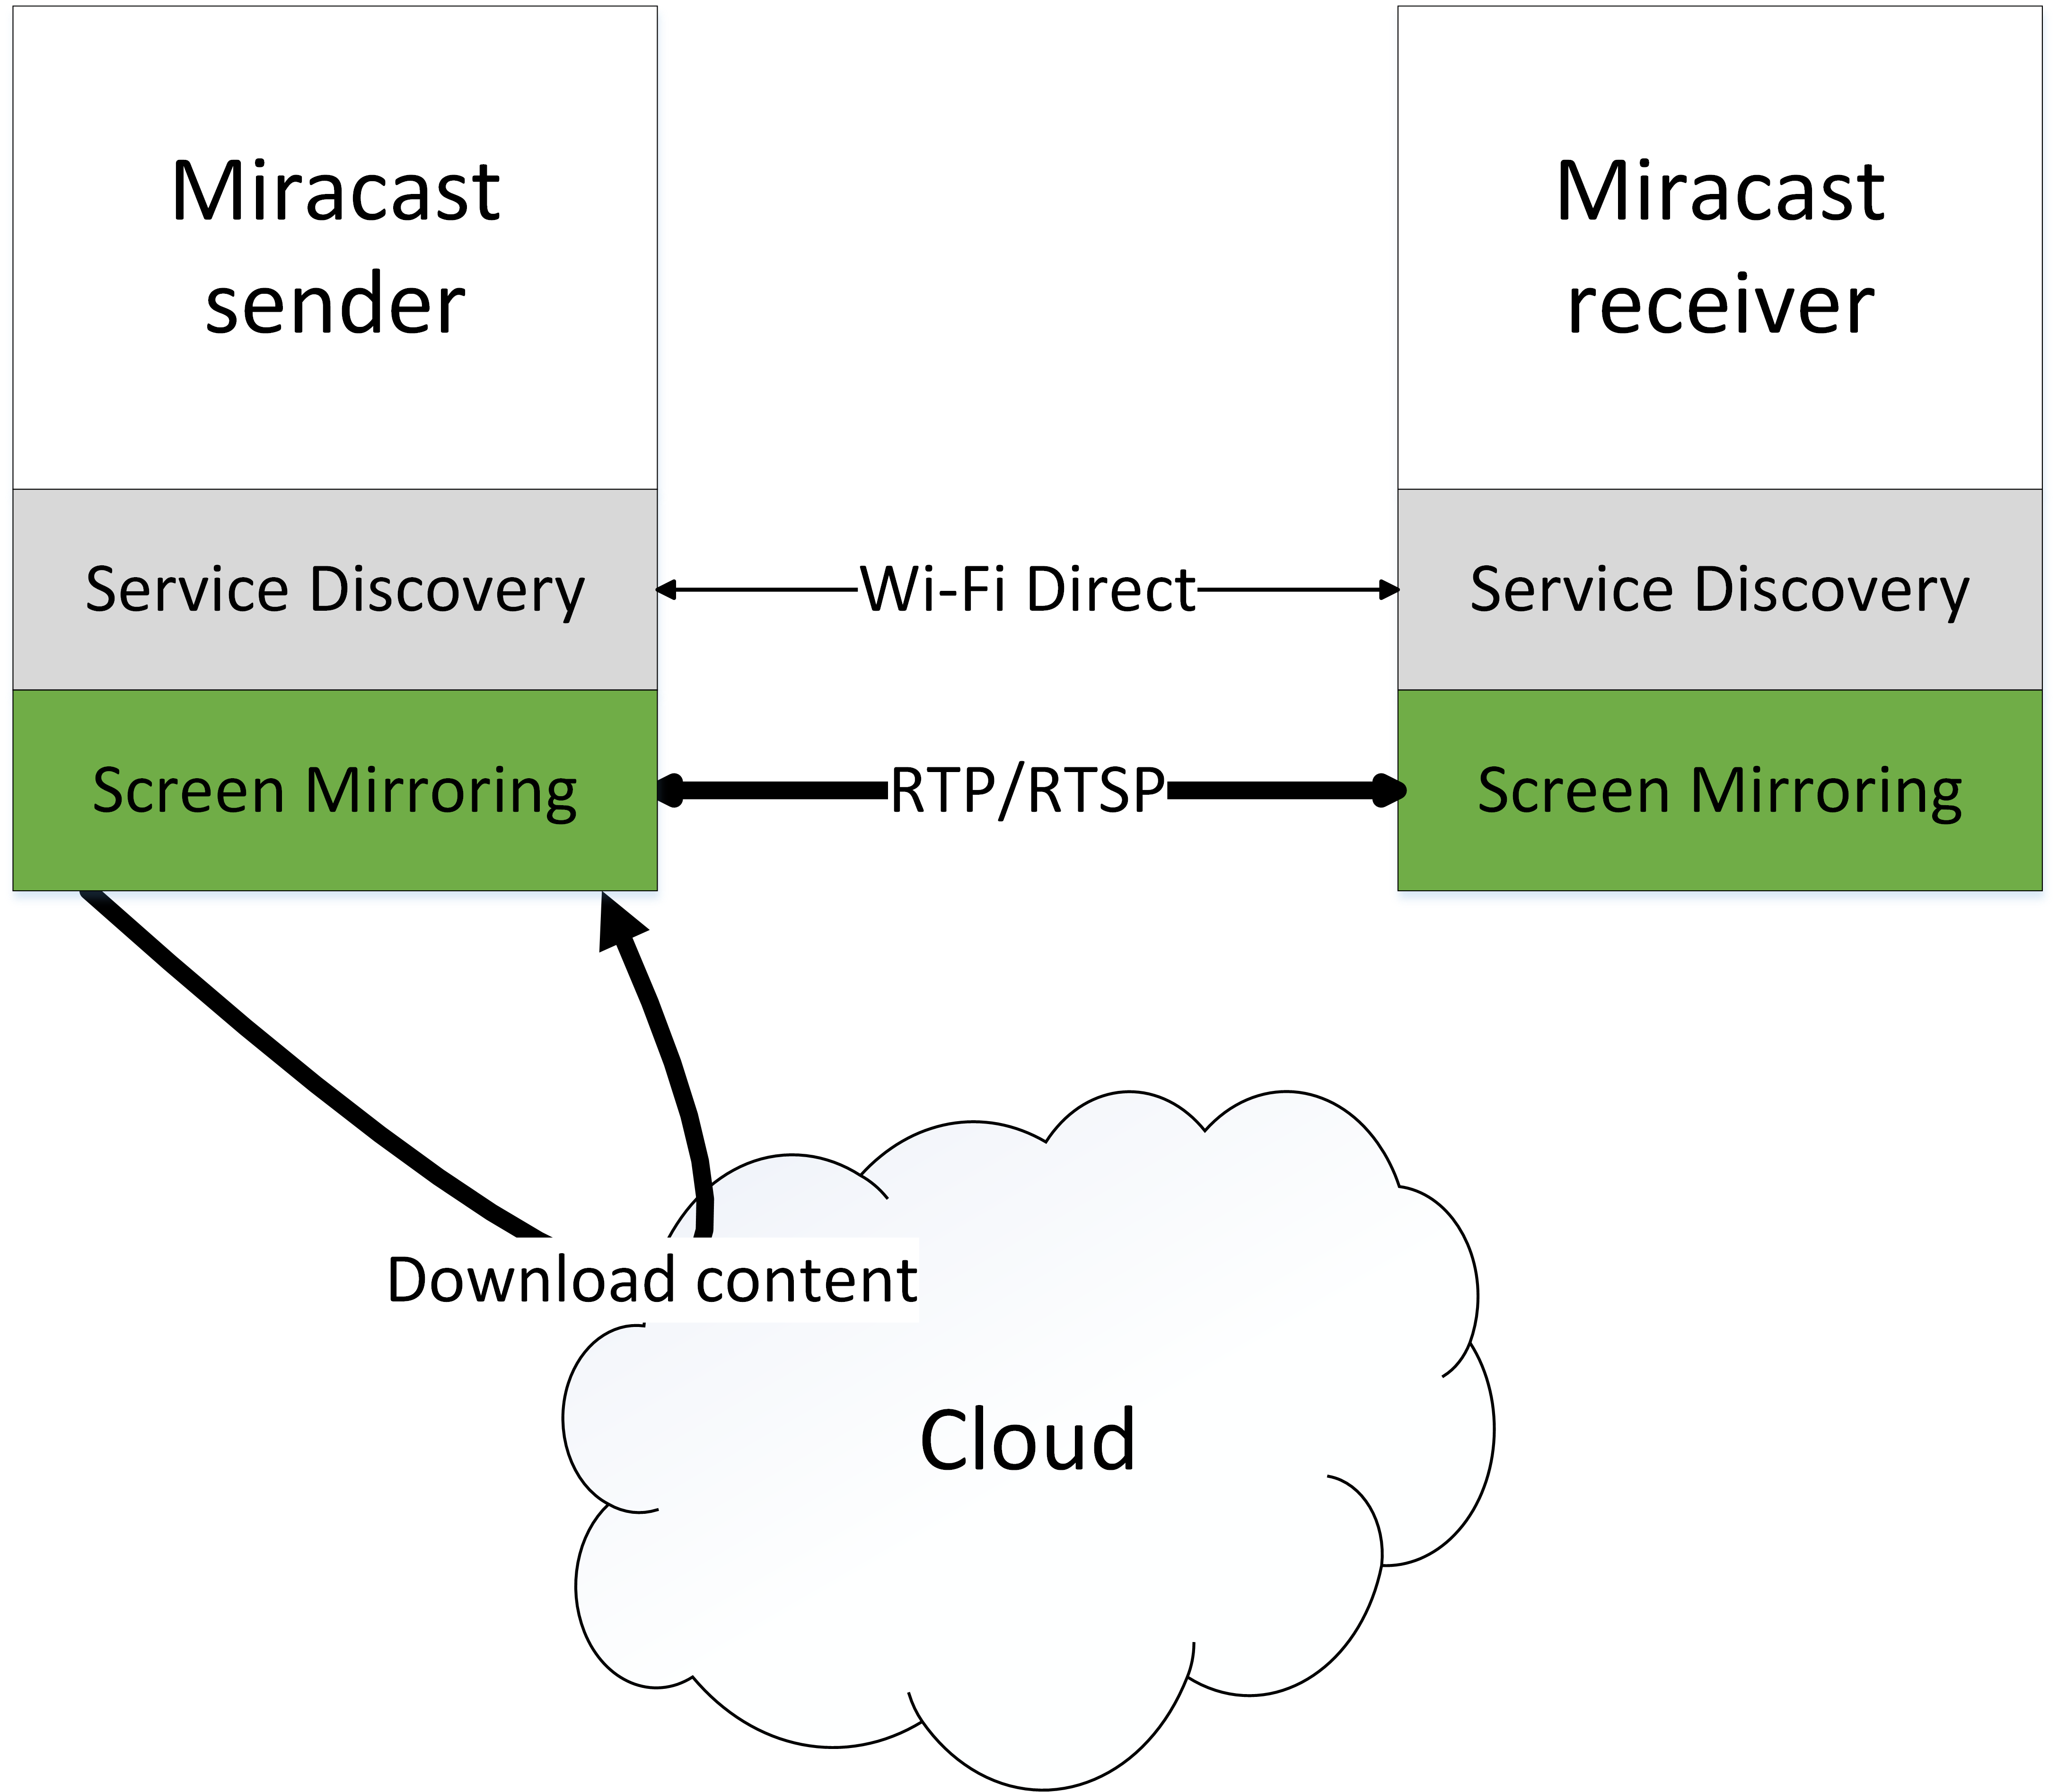
\includegraphics[width=0.7\columnwidth]{charts/miracast} 
\caption{Miracast playback architecture\label{miracast_use_scenario}} 
\end{figure}  

Another point worth mentioning is that Miracast utilizes many Wi-Fi alliance
building blocks that are constantly developed over the years. These components
include Wi-Fi CERTIFIED n (improved throughput and coverage), Wi-Fi Direct
(device-to- device connectivity), Wi-Fi Protected Access 2 (WPA2) (security),
Wi-Fi Multimedia (WMM) (traffic management) and Wi-Fi Protected
Setup \cite{miracast_industry}. These technologies have enriched the user
experience and increased user's trust in Wi-Fi.

Not limited to Wi-Fi direct connection, some Miracast devices also support Tunneled Direct Link Setup (TDLS), which allows devices to connect via an infrastructure network. TDLS enables more efficient data transfer and keeps the advantage of more advanced Wi-Fi capabilities at the same time.

In most cases, Miracast connections are expected to be predominantly established
between Wi-Fi devices connected with each other directly, without an AP acting
as an intermediary. When two devices connect with each other directly, one fulfills its role as the source (the transmitting device) and the other functions as a display (the device receiving and rendering the content to the user).

There are four typical topologies that are supported by Miracast. As shown in
Figure \ref{miracast_model}, the Source could directly connect to the Display
without AP present, or the Source with access to AP and direct connect to the Display, or the source could directly
connect to the Display with AP present, but not connected, or the Source and
the Display could connect to each other and connect to AP at the same time.

On technology perspective, as mentioned previously, Miracast is built upon
many different Wi-Fi technologies. These technologies are built together in an
architecture that can be described by Figure \ref{miracast_architect}.

%% write into article
First of all, the Wi-Fi CERTIFIED n technology provides a transmission channel
designed to support multimedia content. Secondly, Wi-Fi Direct allows devices to
connect directly to each other easily, without the need for a Wi-Fi AP. TDLS
allows devices that are associated to the same Wi-Fi network to establish a
direct link with each other. For security, WPA2 encrypts the transportation
between the source and the display, ensuring the safety of multimedia content.
To guarantee the quality of service (QoS), Wi-Fi Multimedia (WMM) gives real-time
content priority, which is appropriate over best-effort traffic. This brings
better user experience for multimedia content such as video and audio. To
optimize energy consumption, WMM Power Save is used to extend the battery life
of mobile devices by minimizing the time the device is actively connected to
the AP during idle time. Power save mechanisms in Wi-Fi Direct also provide
similar benefits when connecting devices without an AP. Miracast utilizes 
Wi-Fi Protected Setup to increase the ease of use by helping users to
automatically configure Wi-Fi networks, enable WPA2 security, and add new
devices.

The whole Miracast session consists of 10 steps including device discovery,
service discovery, device selection, connection setup, capability negotiation,
content protection setup, session establishment and steaming, user input
channel setup, payload control and display session teardown.

\textbf{Device Discovery}

Source and display devices discover each other prior to connection setup. The Device discovery mechanism is defined in the Wi-Fi Peer-to-Peer (P2P) Specification.

\textbf{Service Discovery}

Source and display devices discover each other's Miracast capabilities prior to connection setup. The Service discovery mechanism is defined in the Wi-Fi P2P specification.

\clearpage

\begin{figure}[htb] \centering 
\hspace*{2cm} 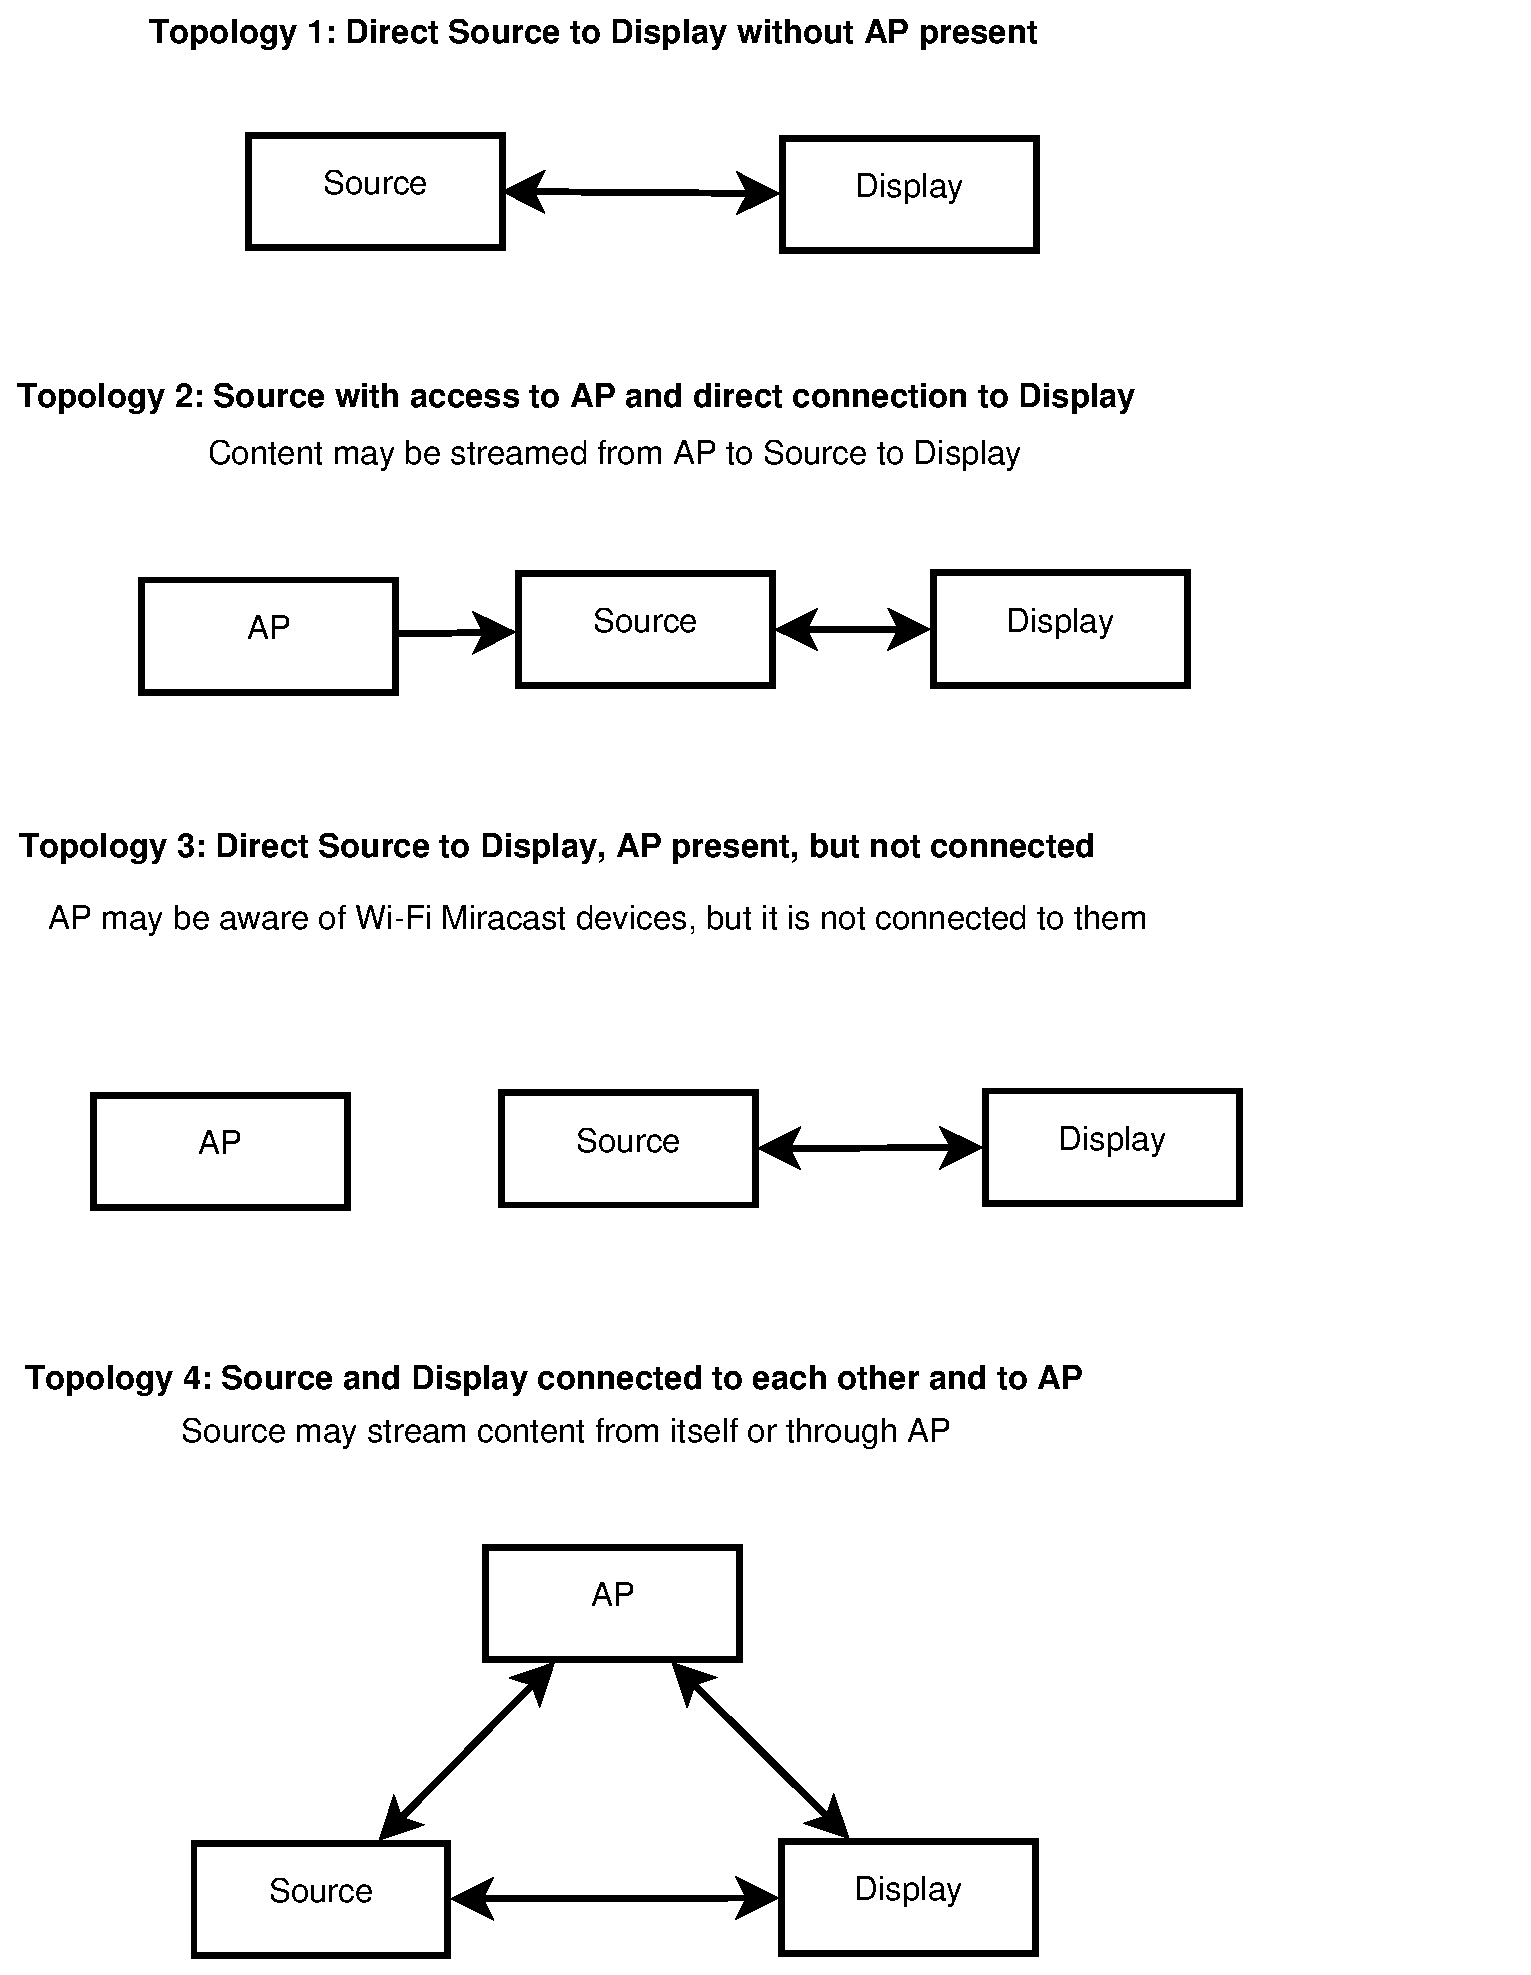
\includegraphics[width=0.9\columnwidth]{charts/miracast_model} 
\caption{Miracast topologies \label{miracast_model}} 
\end{figure} 

\begin{figure}[htb] \centering 
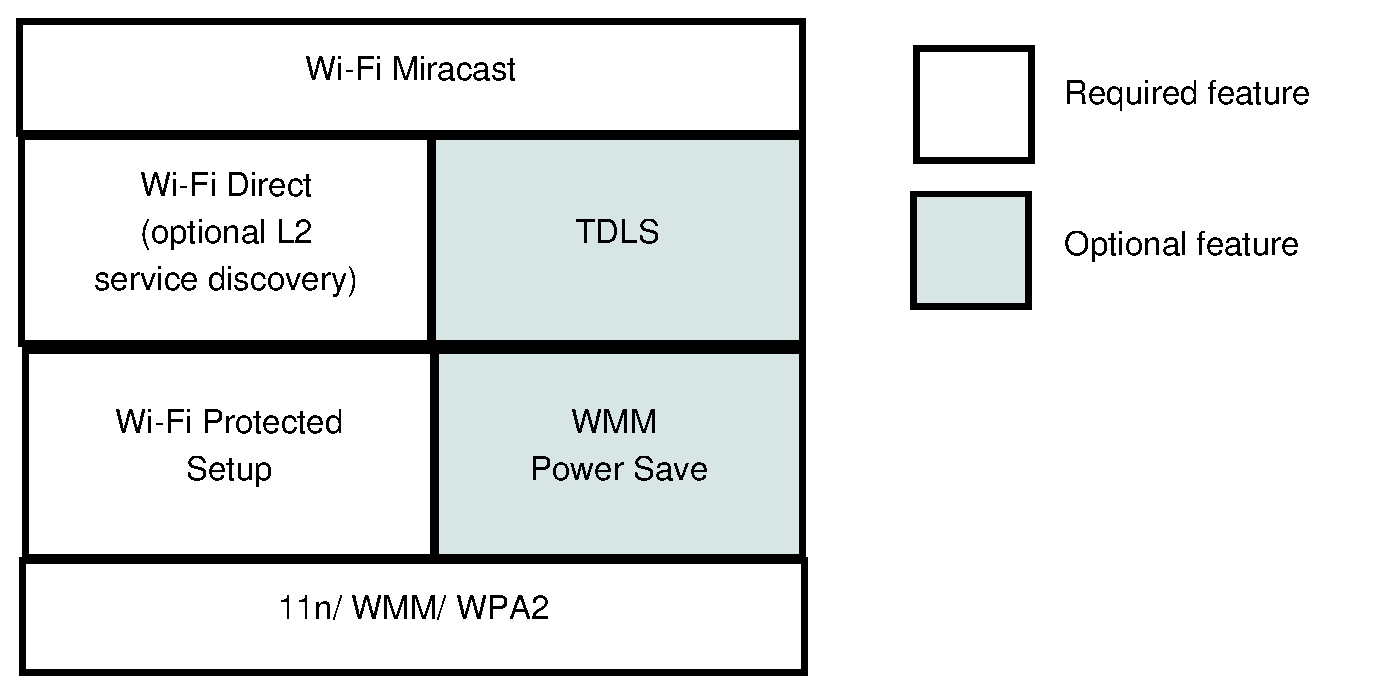
\includegraphics[width=0.9\columnwidth]{charts/miracast_technology_architecture} 
\caption{Miracast technology architecture \label{miracast_architect}} 
\end{figure} 

\textbf{Device selection}

A remote device is selected for connection setup. The user input and the local policies may be used to decide which device is a display and which is a source.

\textbf{Connection setup}

Connection setup selects a method (Wi-Fi Direct or TDLS) to manage the connection. Wi-Fi Direct sets up a group owner and client to initiate a device-to-device link. A WPA2 single-hop link with selected devices is established. Upon the establishment of connectivity between the source and display devices, the display initiates a Transmission Control Protocol (TCP) connection, with a control port using Real-Time Streaming Protocol (RTSP) to create and manage the sessions between the source and the display devices.

\textbf{Capability negotiation} 

Source and display devices determine the parameters for the Miracast session. 

\textbf{Content protection setup (optional)}

If the devices support content protection and their streaming content requires
protection, the session keys for link content protection will be derived using High-bandwidth Digital Content Protection (HDCP) 2.0/2.1. HDCP session keys will be established before the RTP session is initiated. This feature is designed to protect the digital rights of content owners and to encourage the content owner's efforts to make their content available.

\textbf{Session establishment and streaming}

Upon completion of capability negotiation, the source and display devices setup the Miracast session prior to streaming content. The audio and video content available on the source device is packetized 
using Moving Picture Experts Group 2 Transport Stream (MPEG2-TS) coding and
encapsulated by Real-Time Protocol (RTP), User Datagram Protocol (UDP) and Internet Protocol (IP). Finally, IEEE 802.11 packetization enables the source device to send content to the display device.

\textbf{User input back channel setup (optional)}

Optionally, there could be a User Interface Back Channel (UIBC) for transmitting
control and data information related to user interaction with the user interface. User inputs at a display are packetized using a UIBC packet header and transported back using Transmission Control Protocol/Internet Protocol (TCP/IP).

\textbf{Payload control}

When the payload transfer starts, devices may adapt transmission parameters on
the basis of channel conditions and power consumption. Adaptation can be achieved by either compression ratio change and macroblock skipping (using the H.264 standard) or frame skipping (if the display device supports this functionality, the source device may skip some of the frames to be transmitted according to the current resolution) or format change.

\textbf{Display session teardown}

Either the source or the display can terminate the Miracast session.
\subsection{Other protocols\label{2_2_6}}
Apart from all the mentioned standards above, many other companies or associations 
also developed their own proposals, such as
SonosNet\footnote{\url{https://sonos.custhelp.com/app/answers/detail/a_id/126/~/information-about-sonosnet}} that is based on peer to peer network and Spotify Connect 
\footnote{\url{https://www.spotify.com/fi/connect/}}. With all these standards
and proposals competing on the market, the war of standardization on home
networking, however, is still not over.

\subsection{Comparison of existing standards\label{2_3}} 
This section presents the comparison of all the existing solutions discussed in
previous sections, identities the challenges and proposes a solution for
multimedia home networking. Section \ref{2_3_1} describes the evolution history
of the popular home networking solutions. Section \ref{2_3_2} presents the
market share of each standard. Section \ref{2_3_3_1} outlines the supported
media formats of each standard. Section \ref{2_3_3_3} describes the device
diversity of existing solutions which might influence the interoperability.
Section \ref{2_3_3_4} discusses the energy consumption of each solution. Section
\ref{2_3_3_5} compares the features of the existing solutions. Section
\ref{2_3_3_2} summarizes the common protocols used in different standards and
proposes the idea of developing a suitable solution to solve the
incompatibility problem in home networking.
\subsubsection{History\label{2_3_1}} 
DLNA was proposed by several leading consumer electronic manufactures based on
the UPnP technology. From early 2000s on, over 2.2 billion devices with DLNA
have been shipped, making it possible to share audio and video seamlessly among
different smart devices. Moreover, the DLNA alliance had been holding two
meetings annually to discuss the marketing and development related issues,
making DLNA a more and more accomplished standard.

AirPlay, on the other hand, is proposed by Apple Inc. After departing the DLNA alliance in 2010, Apple proposed AirPlay, which brought more advanced features such as screen mirroring, RAOP audio streaming and some authentication functionalities.

Miracast is the most recent technology. It was formerly known as Wi-Fi Display,
which was originally proposed in 2012 by the Wi-Fi alliance. Different from
AirPlay and DLNA, it is not based on home AP but Wi-Fi direct instead. It
provides a screen-mirroring feature that resembles Apple's AirPlay Mirroring.
Now it has gained great popularity among manufactures and software ventures
alike. For instance, Google has launched its Android 4.2 with native support
for Miracast. The latest Kitkat Android 4.4 has even been certified as Miracast
compatible, by the Wi-Fi alliance according to the Wi-Fi Display Specification.
It is now commonly acknowledged that this standard will soon become very
popular in the multi-screen sharing market.

Chromecast or Google cast is another new technology on the market. Released in
2013, a piece of 2.83-inch (72 mm) dongle hardware, which utilizes the DIAL
standard, has become a hot topic recently. With a 35\$ price tag, it has been
ranked as the most popular device of its kind. The DIAL standard was proposed
with the joint effort of Google and Netflix. Since they are Internet companies,
this standard has been designed with Cloud in mind. With the support of the
Cloud, the content is directly streamed from YouTube or Netflix servers to the
Chromecast dongle. One thing worth mentioning is that when using the dongle,
any applications running on mobile platforms are acting as control points. The
dongle provides features like browser mirroring. For example, with a Chromecast
plugin, a Chrome browser can stream its web tab to the dongle that transfers
the signal to a big screen TV. In a foreseeable future, the DIAL standard could
become more and more popular.
\subsubsection{Market\label{2_3_2}} 
DLNA is one of the first proposed solutions for multimedia home 
networking, thus it is so far the most accepted one. Figure 
\ref{dlna_market} shows the history and prediction of the DLNA-certified device sales. In 2018, the 
sales will reach 7.32 billion, nearly the same as the human population on earth.

\begin{figure}[htb] 
\centering 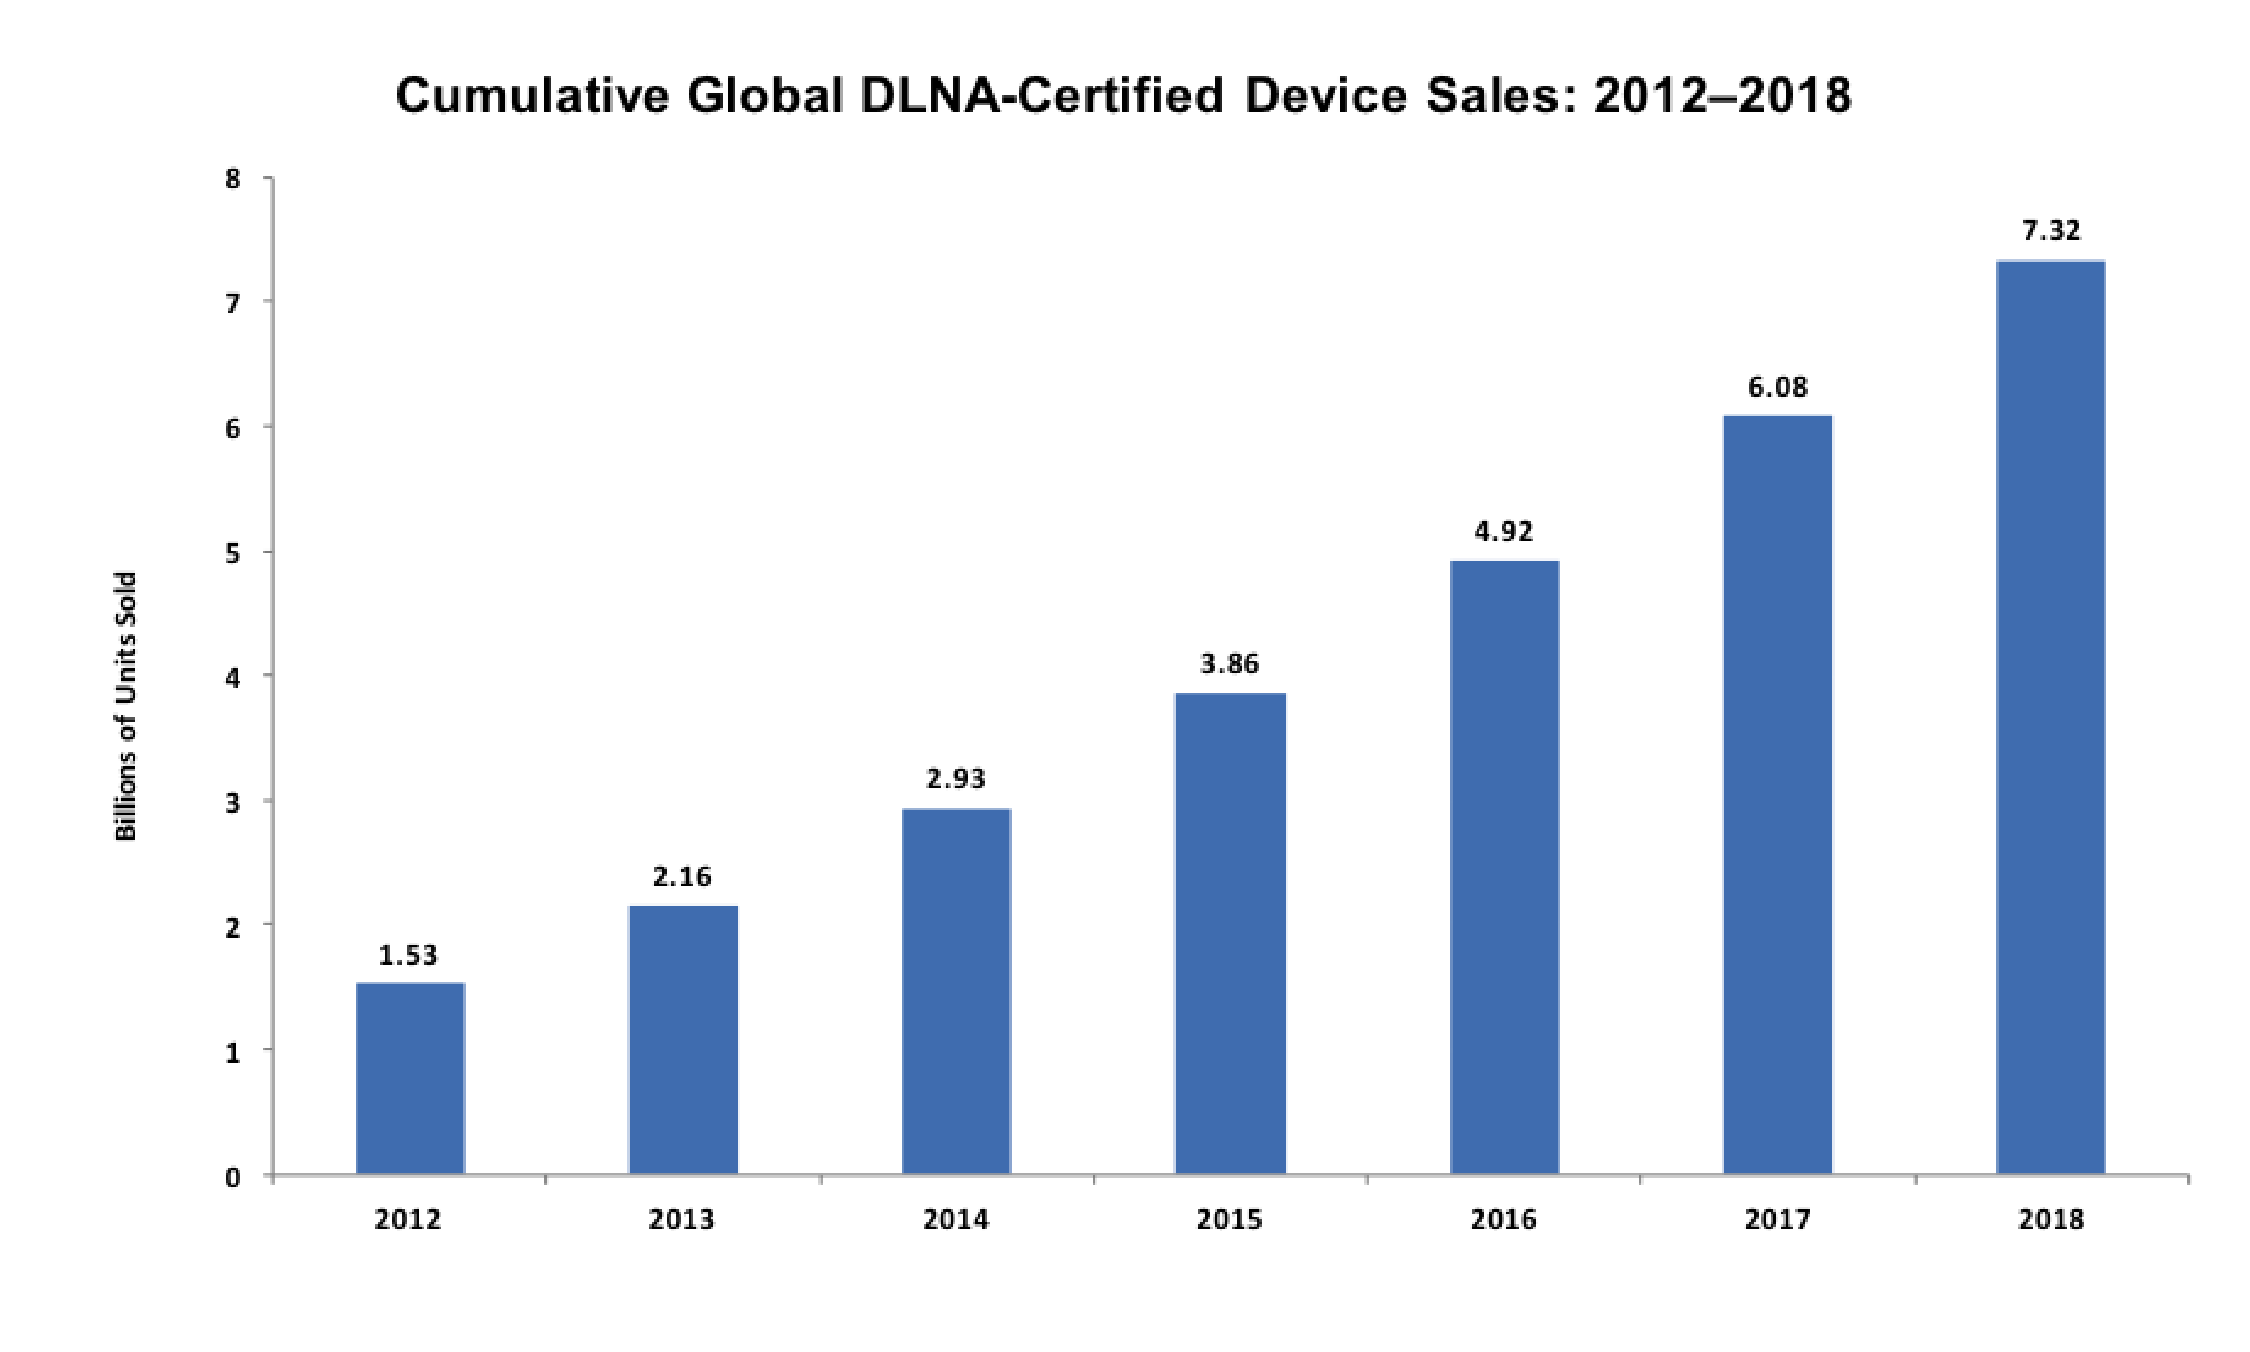
\includegraphics[height=9cm]{charts/dlna_market} 
\caption{Cumulative Global DLNA-Certified Device sales \label{dlna_market}} 
\end{figure}
 
AirPlay is bundled with Apple products. With great sales of Apple TV, Airport Express, 
Mac, iPhone, iPad, iPod, many families have become accustomed to use Apple's
product for everything. In this sense AirPlay has become the easiest way to
build home networking solutions. Moreover, it could be the only solution for
Apple users, since a lot of speaker manufactures implement their own AirPlay
receiver implementations on their AirPlay compatible speakers. And indeed
AirPlay provides enough easy to use features for daily usage.

Bundled with Android operating system, Miracast has experienced a fast growth in 
the past two years. Many latest TVs have been built with Miracast support, to accept peer-to-peer Wi-Fi direct connection.

DIAL standard is used by Chromecast and Amazon Fire TV devices. Chromecast
dongle is a cheap device that everyone wants to try. It can be used to easily
upgrade an old TV to a "Smart TV".  What's more, since Google has provided a
good content support for Chromecast dongle, it has soon been accepted by a huge
amount of users. With the support of Amazon's content and on-line sales
channels, the Amazon Fire TV also attracts a great number of users, especially
in US and UK.

In Chapter \ref{chapter4}, we will have a presentation of the popularity of
different standards according to the statistics of the implemented solution.
\subsubsection{Media format support\label{2_3_3_1}} 
AirPlay and Chromecast have very limited media format support, since there are 
only limited device types. For example, Chromecast has only released 2 devices
so far and there is not much change in the media formats. Similarly Apple TV,
even in its third generation,  has merely seen the improvements in its high
definition support, rather than the changes in media format support.

In contrast, DLNA not only specifies mandatory media formats such as LPCM, JPEG
and MP4, but provides a lot more optional media formats in its specifications
as well.

Since Miracast is a screen mirroring technology, all formats that can be played
on the device are supported in Miracast streaming. Consequently, there is no
mandate on media format in Miracast. Content from
cloud can be downloaded to local device and displayed both on the local device
and receiver device simultaneously, however, it might consume more power
compared with other standards. 
\subsubsection{Device diversity\label{2_3_3_3}}
AirPlay is developed by Apple and mainly used by Apple products. All the latest
iOS devices and OSX devices have embedded the AirPlay sender support. There are
three generations of Apple TV devices available on the market. However,
many speaker manufacturers implemented their own AirPlay music
receivers.

Since DLNA is proposed by several leading electronic companies, and it is
widely accepted as an important standard by the industry, the DLNA devices have
the most diverse implementations among all the introduced standards. There are
billions of DLNA certified devices on the market, which makes the DLNA
compatibility a crucial issue to solve.

Many content providers use the DIAL standard. There are only a few device types
utilizing this standard, such as the Chromecast dongle and Google Nexus Player.
Many content providers, such as YouTube and Netflix, have implemented their own
DIAL channels. Compared with other standards, the implementation guideline of
DIAL standard is strictly defined, so there are not many compatibility issues.

Miracast has become a most widely deployed standard in the last few years. Most
TV models, which are manufactured by Samsung, LG, Sony, have been released with
the Miracast solutions inside. The Miracast support is also integrated into the
latest Android system, which is used by hundreds of mobile phone
models. Although the diversity of devices is significant, the
implementation of Miracast is done by Google and several leading TV
manufacturers. Given this reason, not many compatibility issues are seen for
Miracast.

\subsubsection{Power consumption\label{2_3_3_4}}
As discussed in Section \ref{2_2_2}, since DLNA standard utilizes UPnP AV
architecture, there is a media server device type and a media renderer device
type in the typical use scenario. The streaming traffic is not routed trough
the control point; the energy consumption of the control point is very little.
However, for some use cases, a media server is integrated into a control point;
the power consumption would increase dramatically in this situation. In
addition, most media servers also integrate the transcoding functionality,
which will consume much more power compared with other standards.

For AirPlay, all the streamed music has to be encoded to Apple
Lossless Audio Codec (ALAC) format, which requires the sender to transcode the
most common mp3 or m4a formatted music items, this definitely will consume
significant amount of power. However, when streaming content from online
sources, the traffic can be directly routed to the receiver, the battery
consumption of sender can be preserved.

DIAL, take a Chromecast device as an example, utilizes the cloud as the content
source, for example, Netflix and YouTube videos can be directly routed to the
Chromecast device, the mobile phone only act as a control point.
In this use scenario, even the duration and progress are sent to the control
point through the cloud. This design will significantly reduce the power
consumption of a controller device.

However, Miracast is a screen-mirroring technology, which means the whole
screen will have to be encoded to Moving Picture Experts Group 2 Transport
Stream (MPEG-TS) format, and then sent to a receiver device in real time. This
design will significantly increase the power consumption of the sender device.
Moreover, if the content is from the cloud, the sender device has to download
the content from the cloud, display it on the local screen, and then encode the
whole screen to MPEG-TS format. The whole process will consume the most
significant amount of power compared with all of the introduced standards.
\subsubsection{Features\label{2_3_3_5}}
Compared to some standards, for instance, DLNA, which only provides basic
features, other standards, for example, AirPlay, also offer advanced features,
including screen mirroring. Table \ref{advanced_feature_cmp} below shows the
advanced features provided by different solutions.

%% table 2, compare advance feature 
\begin{table}[htb] 
\caption{Advanced feature comparison \label{advanced_feature_cmp}} 
\begin{center} 
\fbox{ 
\begin{tabular}{c|l|l|l|l}  
\textbf{ } & DLNA & AirPlay & Chromecast & Miracast \\ \hline 
\textbf{Screen mirroring} & No & Yes & No & Yes \\ \hline 
\textbf{Multiple connection} & Yes & No & No & No \\ \hline 
\textbf{Authentication} & No & Yes & No & Yes 
\end{tabular} 
} 
\end{center} 
\end{table} 

\subsubsection{Networking technologies\label{2_3_3_2}}
A short technology specification comparison is made to help better understand
the existing solutions. Table \ref{compare_tech} shows the main technologies
used in different popular solutions.

%% table 1, compare technology 
\begin{table}[htb] 
\caption{Comparison of used technologies\label{compare_tech}} 
\begin{center} 
\fbox{ 
\begin{tabular}{c|l|l|l}  
\textbf{ } & Device discovery & Control Protocol & Streaming protocol \\ \hline 
\textbf{DLNA} & SSDP & UPnP/HTTP & HTTP \\ \hline 
\textbf{AirPlay} & Multicast DNS & HTTP/RTSP & HTTP/RTP \\ \hline 
\textbf{DIAL} & SSDP & DIAL/HTTP & HTTP \\ \hline 
\textbf{Miracast} & Wi-Fi direct & RTSP & RTP 
\end{tabular} 
} 
\end{center} 
\end{table} 

According to the comparison, each standard has its own features and uses 
different protocols to communicate. There are, however, many common features
and protocols that are supported by most standards. For example, the HTTP
protocol is frequently used to handle video and photo streaming, by many
streaming solutions. Another example is that SSDP, the discovery protocol used
by the UPnP devices, is commonly used for device discovery for many other
standards.

Since multiple standards share the commonly used protocols in their
implementations, it is possible to make an application that is aware of all
these common protocols. In this sense, making such a mobile application to
connect multiple types of devices in a home network can be a good solution to
home-networking interoperability. With such an application, contents from
different sources will be able to be streamed to different receivers regardless
of their standards, which makes multimedia home networking more convenient to
use for end users.